\documentclass[12pt,a4paper]{article}

\usepackage{amsmath}
\usepackage[dutch]{babel}
\usepackage{hyperref}
\usepackage{enumerate}
\usepackage{graphicx}
\usepackage{float}
\usepackage{listings}
\usepackage{subfig}
\usepackage{color}
\definecolor{lightgray}{rgb}{.9,.9,.9}
\definecolor{darkgray}{rgb}{.4,.4,.4}
\definecolor{purple}{rgb}{0.65, 0.12, 0.82}
\renewcommand\lstlistingname{Programma}
\renewcommand\lstlistlistingname{Programma}

\lstdefinelanguage{Javascript}{
  keywords={typeof, new, true, false, catch, function, return, null, catch, switch, var, if, in, while, do, else, case, break},
  keywordstyle=\color{blue}\bfseries,
  ndkeywords={class, export, boolean, throw, implements, import, this},
  ndkeywordstyle=\color{darkgray}\bfseries,
  identifierstyle=\color{black},
  sensitive=false,
  comment=[l]{//},
  morecomment=[s]{/*}{*/},
  commentstyle=\color{purple}\ttfamily,
  stringstyle=\color{red}\ttfamily,
  morestring=[b]',
  morestring=[b]"
}

\lstset{
   language=JavaScript,
   extendedchars=true,
   basicstyle=\footnotesize\ttfamily,
   showstringspaces=false,
   showspaces=false,
   numbers=left,
   numberstyle=\footnotesize,
   numbersep=9pt,
   tabsize=2,
   breaklines=true,
   showtabs=false,
   captionpos=b
}

\title{Een fysisch systeem voor de computer}
\date{\today}
\author{Derk Rouwhorst en Harmen Stoppels}

\begin{document}
	\begin{titlepage}
		\maketitle
		\thispagestyle{empty}
	\end{titlepage}

	\tableofcontents
	\newpage
	
	\section{Voorwoord}
	Dit profielwerkstuk is gemaakt in het kader van het profiel Natuur en Techniek, en is vooral een verbreding in de vakken natuurkunde, wiskunde en informatica. Dit is het schriftelijk eindproduct, waarin we verslag doen van ons onderzoek naar tweedimensionale botsingen en het schrijven van een simulatieprogramma. Naast het schriftelijk eindproduct is een USB-stick bijgeleverd met het offici\"{e}le eindproduct.
	
	Derk Rouwhorst heeft zich vooral gericht op de praktische kant, zoals het onderzoeken van een praktijkvoorbeeld en daarna het uitzoeken wat het gevolg van botsingen is, met behulp van formules. Harmen Stoppels heeft zich vooral gericht op de theoretische kant, zoals het opstellen van vergelijkingen voor tijdstippen van botsingen en het programmeren van het eindproduct.
	
	We bedanken meneer Prins voor het begeleiden van het project, meneer Leemhuis voor hulp bij het prakticum en het uitlenen van apparatuur, en als laatste meneer Stoppels voor uitleg en hulp bij het opstellen van vergelijkingen.
	
	\newpage
		
	\section{Inleiding}
	Wij hebben ervoor gekozen om een fysisch systeem te maken voor de computer, waarmee onder andere tweedimensionale botsingen gesimuleerd kunnen worden. Onze hoofdvraag hierbij is:
	\\
	\\\textbf{Hoe maken we een fysisch systeem dat tweedimensionale botsingen kan simuleren?}
	\\
	\\Daarbij hebben we de volgende deelvragen bedacht:

	\begin{enumerate}
		\item Hoe werken botsingen bij poolballen?
		\item Met welke natuurkundige en wiskundige formules is de beweging te beschrijven?
		\item Hoe programmeer je deze formules?
		\item Hoe optimaliseer je de snelheid van het programma?
	\end{enumerate}

	Omdat de berekening grotendeels gebeuren met behulp van vectoren, geven we eerst een uitleg over vectoren. Op het moment van botsen veranderen de snelheid en de richting van de ballen. Maar eerst moet je weten op welk tijdstip dat gebeurt en wat dan de snelheden en de posities zijn. Het bepalen van dat moment leggen we ook uit, hierbij moet onderscheid gemaakt worden tussen botsingen tussen ballen en botsingen met een bal en een lijnstuk. Er zit ook veel natuurkundige theorie achter botsingen. Dit leggen we eerst uit voordat we aan de botsingen gaan rekenen. Het resultaat kan op meerdere manieren verkregen worden, hier behandelen we twee manieren. De eerste manier gaat met behulp van de wet van behoud van energie en de wet van behoud van impuls. De tweede manier werkt ook met de wet van behoud van impuls een maakt gebruik van de gemeenschappelijke snelheid. Deze tweede manier is aanzienlijk korter. Met al deze informatie en formules is het programma gemaakt. We zullen niet het hele programma stap voor stap verklaren, maar samenvatten en in grote lijnen vertellen wat er gebeurt.

	\newpage
	
	\section{Vectoren}
	We drukken in ons hele profielwerkstuk snelheden, posities en krachten zoveel mogelijk uit in vectoren. Hiermee maken we het rekenwerk een stuk makkelijker en kunnen we formules veel korter opschrijven. We maken gebruik van tweedimensionale vectoren, die uit een $x$- en een $y$-component in het cartesisch co\"{o}rdinatenstelsel bestaan. In de voorbeelden en definities in dit onderdeel gebruiken we alleen tweedimensionale vectoren, ook al gelden veel ervan ook voor $n$-dimensionale vectoren.
	
	\subsection{Notatie}
	De namen van vectoren schrijven we dikgedrukt en de componenten boven elkaar met ronde haken eromheen. Een voorbeeld hiervan is $\mathbf{v} = \begin{pmatrix} v_1 \\ v_2 \end{pmatrix} = \begin{pmatrix} 5 \\ -3 \end{pmatrix}$. Dit stelt een vector voor die $5$ naar rechts is gericht en $3$ naar onder.
	
	\subsection{Norm van een vector}
	De norm van een vector is de lengte of grootte. Deze wordt aangeduid met een dubbele verticale streep rondom de vector. Oftewel, de norm van vector $\mathbf{v}$ is $\|\mathbf{v}\| = \sqrt{{v_1}^2+{v_2}^2}$.
	
	\subsection{Eenheidsvector}
	Een eenheidsvector is een vector waarvan de norm 1 is. Het handige van zo'n vector is dat hij, vermenigvuldigd met een getal, zijn richting behoudt en de norm van het getal waarmee vermenigvuldigd is aanneemt. Stel, je hebt de richting waarin een voorwerp beweegt als eenheidsvector, dan geeft vermenigvuldiging met de snelheid, de snelheid als vector. De notatie van de eenheidsvector wordt gedaan met een dakje erop: $\|\mathbf{\hat{a}}\| = 1$.
	
	\subsection{Het inwendig product}
	Het inwendig product van twee vectoren is de som van alle componenten met elkaar vermenigvuldigd. Een voorbeeld hiervan is:
	
	\begin{equation*}
		\begin{aligned}
			\mathbf{v} &= \begin{pmatrix} 5 \\ -3 \end{pmatrix}, \mathbf{u} = \begin{pmatrix} 4 \\ 2 \end{pmatrix} \\
			\mathbf{v} \cdot \mathbf{u} &= 5 \times 4 -3 \times 2 = 14\\
		\end{aligned}
	\end{equation*}
	
	Deze rekenkundige bewerking blijkt heel goed toepasbaar te zijn in geometrische berekeningen. We gebruiken het inproduct onder andere om een vector op een andere te projecteren, en ook om te kijken of een voorwerp een lijnstuk of juist de lijn in het verlengde van het lijnstuk raakt.

	Werken met het inproduct zorgt niet alleen voor een kortere notatie, maar blijkt ook in sommige gevallen de voor de computer tijdrovende functie cosinus te vervangen.
	
	Het bewijs voor de laatstgenoemde eigenschap maakt gebruik van de cosinusregel. Gegeven zijn de vectoren $\mathbf{a}=\begin{pmatrix} a_1 \\ a_2 \end{pmatrix}$ en $\mathbf{b}=\begin{pmatrix} b_1 \\ b_2 \end{pmatrix}$ met hetzelfde beginpunt en een onderlinge hoek $\gamma$ en vector $\mathbf{c}$ tussen beide uiteinden van $\mathbf{a}$ en $\mathbf{b}$. Zie figuur \ref{cosinusregel-inproduct}.
	
	\begin{figure}[h]
		\centerline{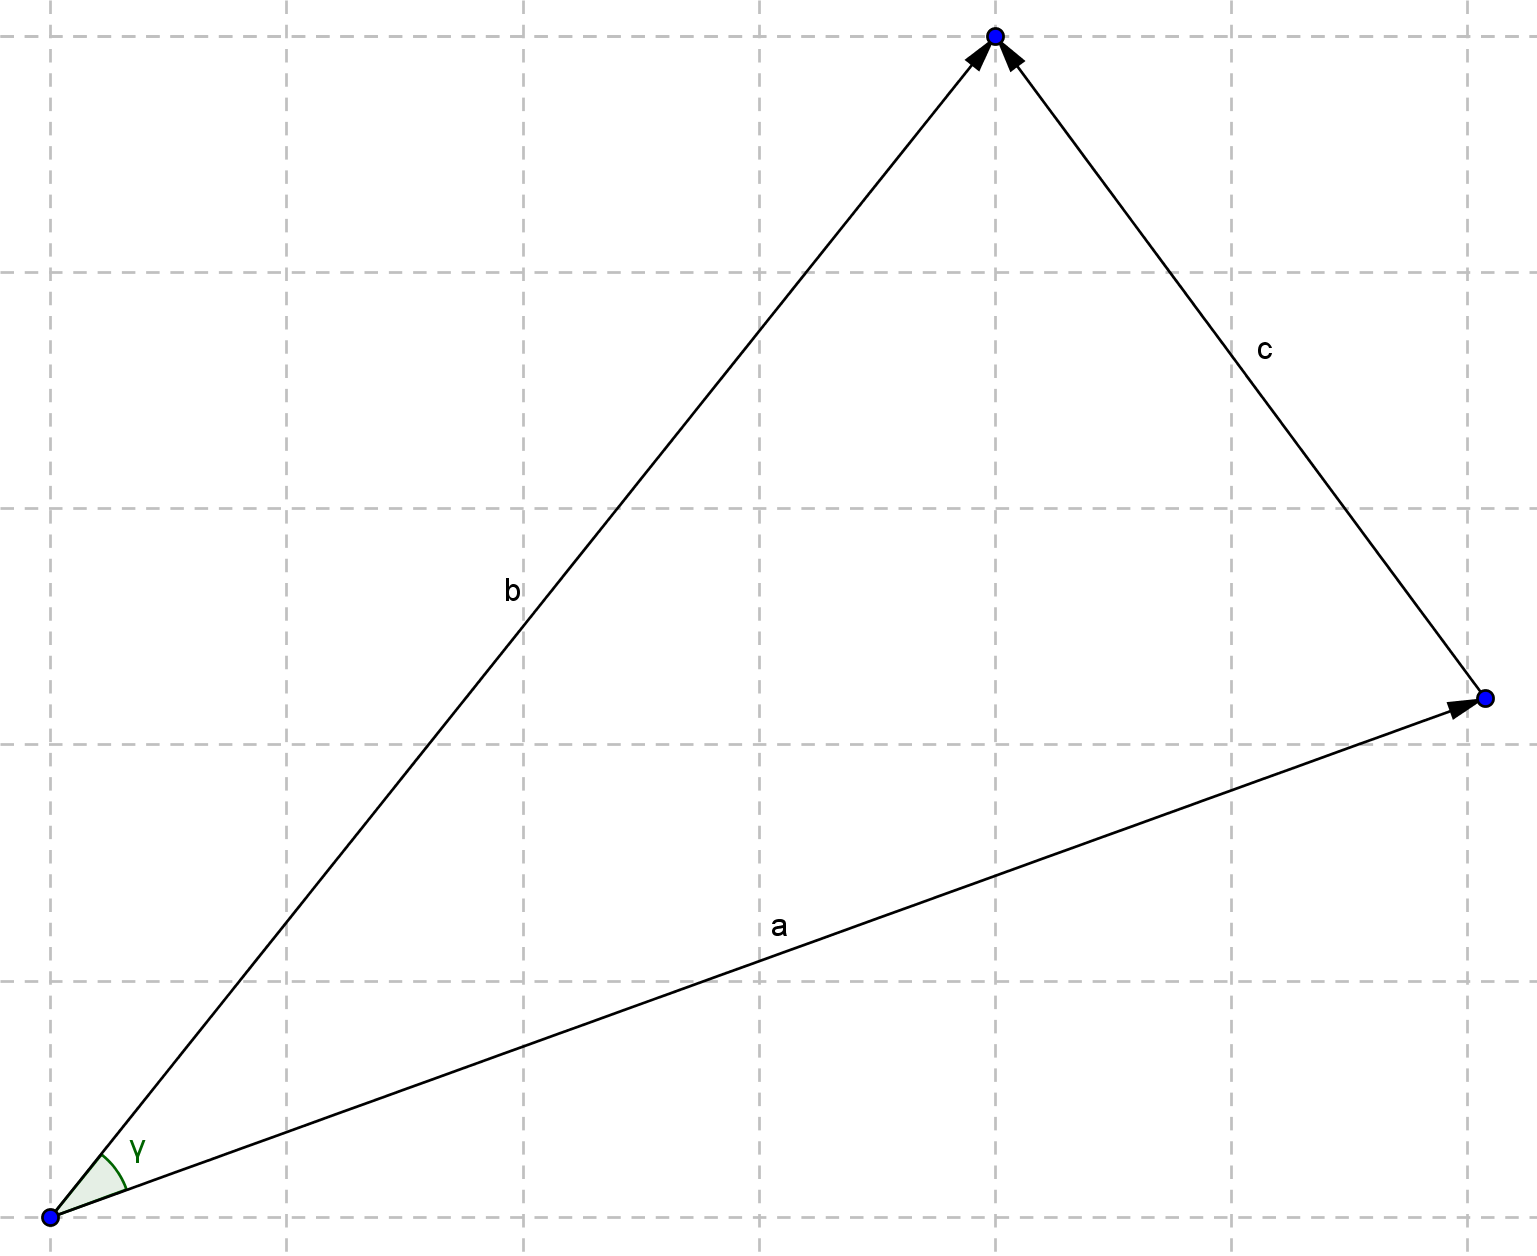
\includegraphics[width=\textwidth]{Plaatjes/cosinusregel-inproduct.png}}
		\caption{Een driehoek met vectoren als zijden}
		\label{cosinusregel-inproduct}
	\end{figure}
	
	Voor de lengte van vector $\mathbf{c}$ geldt dan:
 	\begin{equation}
		\begin{aligned}
			\|\mathbf{c}\|^2 = \left\{ 
				\begin{array}{l l}
 	 				(a_1-b_1)^2+(a_2-b_2)^2 \\
  					{\|\mathbf{a}\|}^2 + {\|\mathbf{b}\|}^2 - 2 \cdot \|\mathbf{a}\| \cdot \|\mathbf{b}\| \cdot \cos\gamma 
 	 			\end{array} 
 	 		\right.
		\end{aligned}
	\end{equation}
	\\Hieruit volgt:
	\begin{equation}
		\label{inproduct-cosinus}
		\begin{aligned}
			(a_1-b_1)^2 + (a_2-b_2)^2 &= {\|\mathbf{a}\|}^2 + {\|\mathbf{b}\|}^2 - 2 \cdot {\|\mathbf{a}\|} \cdot {\|\mathbf{b}\|} \cdot \cos\gamma \\
			{a_1}^2 + {a_2}^2+ {b_1}^2 + {b_2}^2 - 2a_1b_1 - 2a_2b_2 &= {a_1}^2 + {a_2}^2+ {b_1}^2 + {b_2}^2 - 2 \cdot {\|\mathbf{a}\|} \cdot {\|\mathbf{b}\|} \cdot \cos\gamma \\
			-2a_1b_1 - 2a_2b_2 &= - 2 \cdot {\|\mathbf{a}\|} \cdot {\|\mathbf{b}\|} \cdot \cos\gamma \\
			-2(a_1b_1 + a_2b_2) &= - 2 \cdot {\|\mathbf{a}\|} \cdot {\|\mathbf{b}\|} \cdot \cos\gamma \\
			-2(\mathbf{a} \cdot \mathbf{b}) &= - 2 \cdot \|\mathbf{a}\| \cdot \|\mathbf{b}\| \cdot \cos\gamma \\
			\mathbf{a} \cdot \mathbf{b} &= \|\mathbf{a}\| \cdot \|\mathbf{b}\| \cdot \cos\gamma\\
		\end{aligned}
	\end{equation}
	
	\subsection{Normaalvector}
	De normaalvector van een vector is de vector die loodrecht op de andere vector staat. Een normaalvector is makkelijk af te leiden, algemeen geldt: als vector $\mathbf{v}=\begin{pmatrix} v_1 \\ v_2 \end{pmatrix}$ is gegeven, dan is de normaalvector $\mathbf{n}=\begin{pmatrix} -v_2 \\ v_1 \end{pmatrix}$.
	
	Het inproduct van een vector met zijn normaalvector is altijd 0, bijvoorbeeld:
	
	\begin{equation}
		\begin{aligned}
			\mathbf{v} &= \begin{pmatrix} 4 \\ 2 \end{pmatrix}\\
			\mathbf{n} &= \begin{pmatrix} -2 \\ 4 \end{pmatrix} \\
			\mathbf{v} \cdot \mathbf{n} &= 4 \cdot -2 + 2 \cdot 4 = 0
		\end{aligned}
	\end{equation}
	
	Dit volgt ook uit de eigenschap van het inproduct \eqref{inproduct-cosinus}, de cosinus van 90 graden is namelijk 0.

	\newpage

	\section{Tijdstippen van botsingen}
	
	\subsection{Cirkel tegen cirkel}
	Kijken of twee stilstaande cirkels elkaar raken is theoretisch erg makkelijk te doen. Het komt er simpelweg op neer dat de cirkels elkaar raken als de som van de stralen gelijk is aan de afstand tussen de middelpunten. Het wordt echter lastiger als de cirkels bewegen en elkaar in een simulatie tussen twee frames raken. Het probleem is dat het gros van de botsingen tussen bewegende cirkels juist tussen twee frames gebeurt.
	
	\subsubsection{Formule}
	\begin{figure}[h]
		\centerline{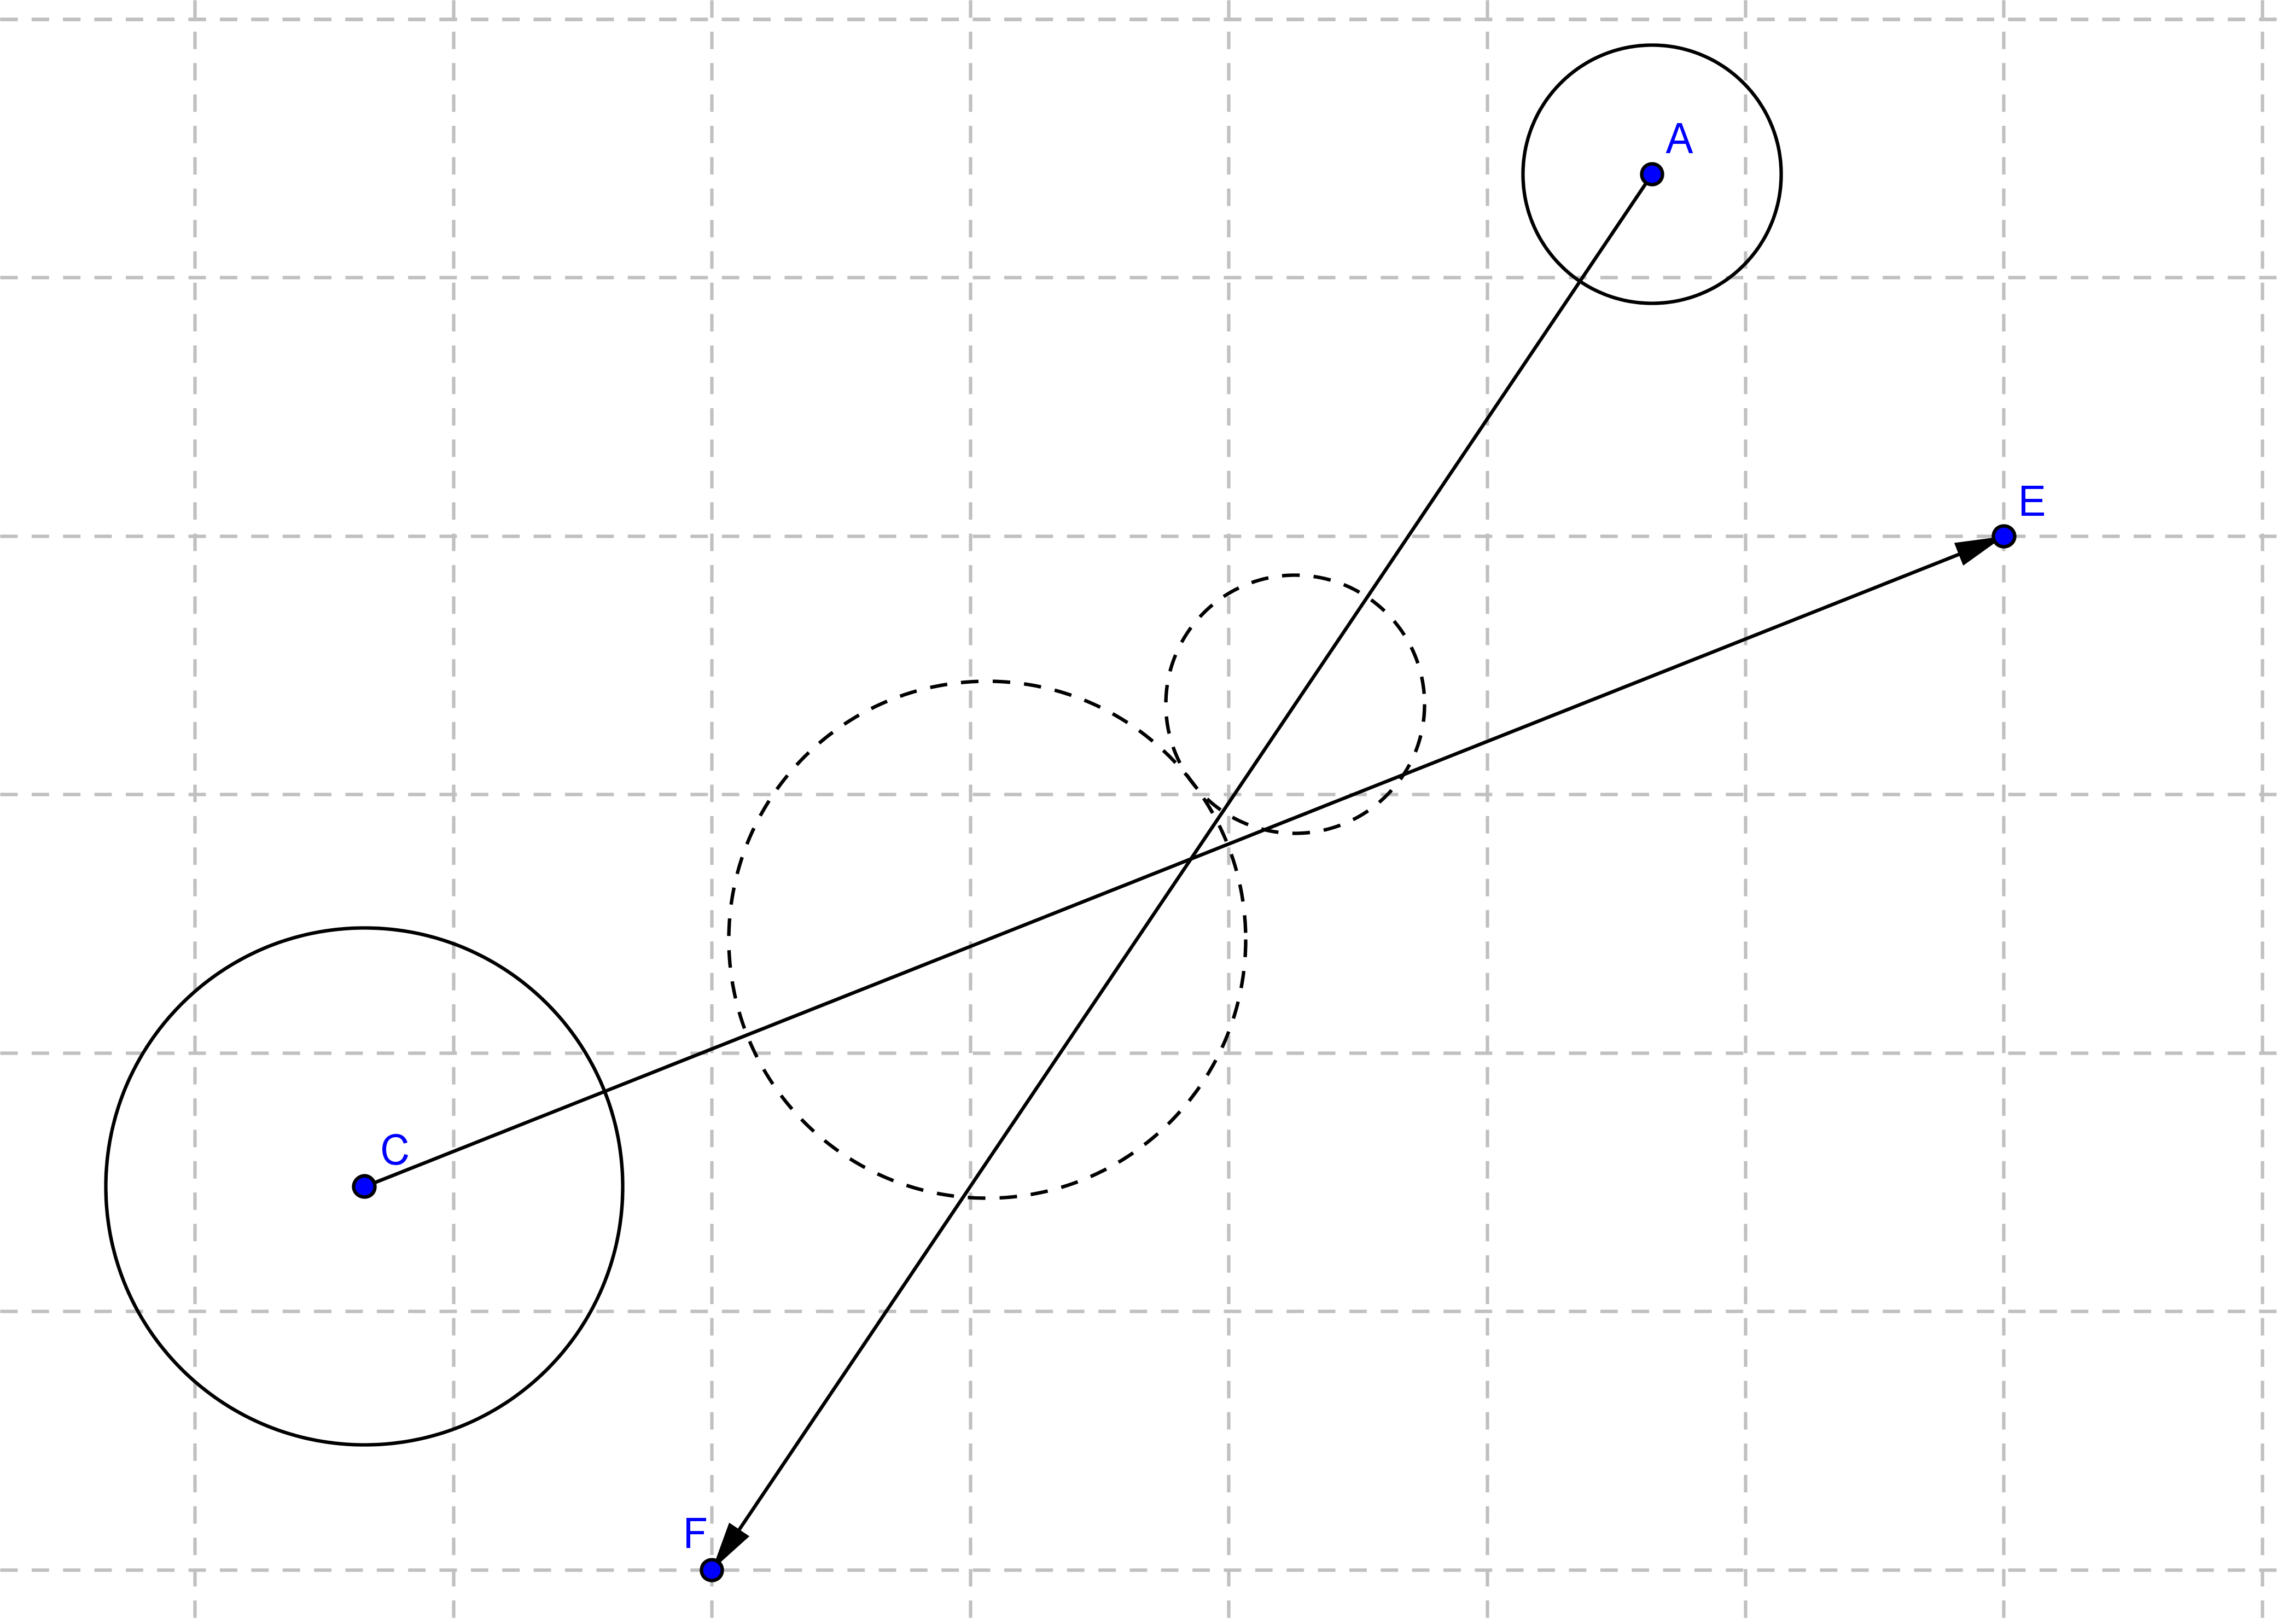
\includegraphics[width=\textwidth]{Plaatjes/Bal-Bal.png}}
		\caption{Hoe bereken je op welk moment twee bewegende ballen botsen?}
		\label{bal-bal}
	\end{figure}
	
	Bij het berekenen van de nieuwe posities van de ballen in het volgende frame, moeten we dus als eerste kijken of ze ondertussen botsen, als tweede berekenen wanneer dat is en als derde uitvinden wat voor gevolg die botsing heeft.
	
	Om de uiteindelijke vergelijking te versimpelen gaan wij ervan uit dat elk voorwerp tussen twee frames een constante snelheid heeft en over een rechte lijn beweegt. Dit klopt niet met de realiteit, maar omdat de tijd tussen twee frames erg klein is, maakt het niet zo veel uit. Zie ook paragraaf \ref{werking-van-het-programma}.
	
	De cirkels kunnen elkaar op het tijdsinterval tussen twee frames hoogstens twee keer raken (geen rekening gehouden met het effect van de botsing), namelijk wanneer ze voor het eerst tegen elkaar aankomen en wanneer ze door elkaar heen zijn gevlogen. De botsing die wij moeten vinden is de eerste, de tweede vindt natuurlijk nooit plaats.
	
	Allereerst noemen we de tijd in het eerste frame $t=0$ en in het tweede frame $t=1$. We zoeken een waarde van $t$ waarvoor geldt dat $0 \le t < 1$ en waarbij de afstand tussen de middelpunten gelijk is aan de som van de stralen.
	
	De posities van de ballen geven we aan met vectoren. De nieuwe positie bestaat uit de oude positie met daarbij opgeteld de snelheidsvector vermenigvuldigd met de tijd. Wat we krijgen is dus:
	\begin{equation}
		\begin{aligned}
			\mathbf{X} &:= \mathbf{X} + \mathbf{v}t\\
		\end{aligned}
	\end{equation}
	\\Vul je $t=0$ in, dan krijg je de positie in frame 1; vul je $t=1$, dan krijg je de positie in frame 2, als er tussendoor geen botsing plaatsvindt.
	
	We moeten nu een vergelijking opstellen en oplossen voor $t$, waarin we de relatieve afstand tussen twee ballen gelijkstellen aan de som van de stralen:
	
	\begin{equation}
		\begin{aligned}
			 \|\mathbf{X_1} + \mathbf{v_1}t  - \mathbf{X_2} -  \mathbf{v_2}t \| &= r_1 + r_2 \\
			 \|\mathbf{X_{rel}} + \mathbf{v_{rel}}t \| &= r_1 + r_2\\
		\end{aligned}
	\end{equation}
	\\Beide kanten kwadrateren geeft:
	\begin{equation}
		\label{botsing}
		\begin{aligned}
			\mathbf{v_{rel}}^2 t^2 + 2 \mathbf{X_{rel}} \mathbf{v_{rel}} + \mathbf{X_{rel}}^2  &= (r_1 + r_2)^2 \\
			(\mathbf{v_{rel}} \cdot \mathbf{v_{rel}})t^2 + 2(\mathbf{X_{rel}} \cdot \mathbf{v_{rel}})t + \mathbf{X_{rel}} \cdot \mathbf{X_{rel}} &= (r_1 + r_2)^2 \\
			(\mathbf{v_{rel}} \cdot \mathbf{v_{rel}})t^2 + 2(\mathbf{X_{rel}} \cdot \mathbf{v_{rel}})t + \mathbf{X_{rel}} \cdot \mathbf{X_{rel}} - (r_1 + r_2)^2 &= 0\\
		\end{aligned}
	\end{equation}
	\\Deze vergelijking is een eenvoudige vierkantsvergelijking en kan met de ABC-formule worden opgelost, maar we kiezen ervoor om een iets alternatieve vorm de ABC-formule te gebruiken om de rekentijd te beperken:
	
	\begin{equation}
		\label{a2bc}
		\begin{aligned}
			at^2+2bt+c &= 0 \\
			t^2+\tfrac{2b}{a}t &= -\frac{c}{a} \\
			\left( t+\tfrac{b}{a} \right)^2 &= \frac{b^2}{a^2} -\frac{c}{a} \\
			t + \tfrac{b}{a} &= \pm \sqrt{\frac{b^2 - ac}{a^2}} \\
			t &= \frac{-b \pm \sqrt{b^2 - ac}}{a}\\
		\end{aligned}
	\end{equation}
	\\Vergelijking \eqref{a2bc} kunnen we nu toepassen op vergelijking \eqref{botsing}:
	
	\begin{equation}
		\begin{aligned}
			a &= \mathbf{v_{rel}} \cdot \mathbf{v_{rel}} \\
			b &= \mathbf{X_{rel}} \cdot \mathbf{v_{rel}} \\
			c &= \mathbf{X_{rel}} \cdot \mathbf{X_{rel}} - (r_1 + r_2)^2\\
		\end{aligned}
	\end{equation}
	
	\subsubsection{Simulatie}
	We hebben deze formule omgezet naar een simulatie in \href{http://www.geogebra.org/webstart/geogebra.html}{Geogebra}, om te kijken of de formule klopte. Zie de bijlage met de bestandsnaam Bal-Bal.ggb. Zowel de verplaatsingsvectoren, beginposities en de stralen van beide cirkels zijn aan te passen, en als er binnen het begin- en eindpunt een botsing is, worden de cirkels opnieuw gestippeld getekend op de plaats van de botsing.
	
	\subsection{Cirkel tegen lijnstuk}
	De vergelijking die we moeten opstellen om te kijken of een cirkel binnen een tijdsinterval van \'{e}\'{e}n frame botst met een lijnstuk is lastiger dan dat van twee cirkels. Het is namelijk een stuk lastiger om de kortste afstand tussen een cirkel en een lijnstuk te vinden, maar het we hebben wel een elegante oplossing gevonden.
	
	\subsubsection{Tijdstippen van botsingen}
	Gegeven is een lijnstuk $AB$ en een cirkel die met constante snelheid over lijnstuk $CD$ beweegt. De cirkel heeft straal $r$ en botst tijdens zijn beweging misschien tegen lijnstuk $AB$. Op tijdstip $t=0$ bevindt het middelpunt van de cirkel zich op $C$, op tijdstip $t=1$ bevindt het zich op $D$. We zoeken naar de eerste waarde voor $t$ tussen $0$ en $1$ waarop de cirkel lijnstuk $AB$ raakt.
	
	Om dit probleem op te lossen gebruiken we een vergelijking voor de afstand van een punt tot een lijn, en die afstand moet gelijk zijn aan de straal van de cirkel. Als $AB$ en $CD$ niet parallel lopen, krijgen we twee oplossingen voor onze vergelijking. De eerste is de botsing, de tweede oplossing geeft het tijdstip aan waarop de cirkel door $AB$ is gevlogen en het lijnstuk dan raakt.
	
	\begin{figure}[h]
		\centerline{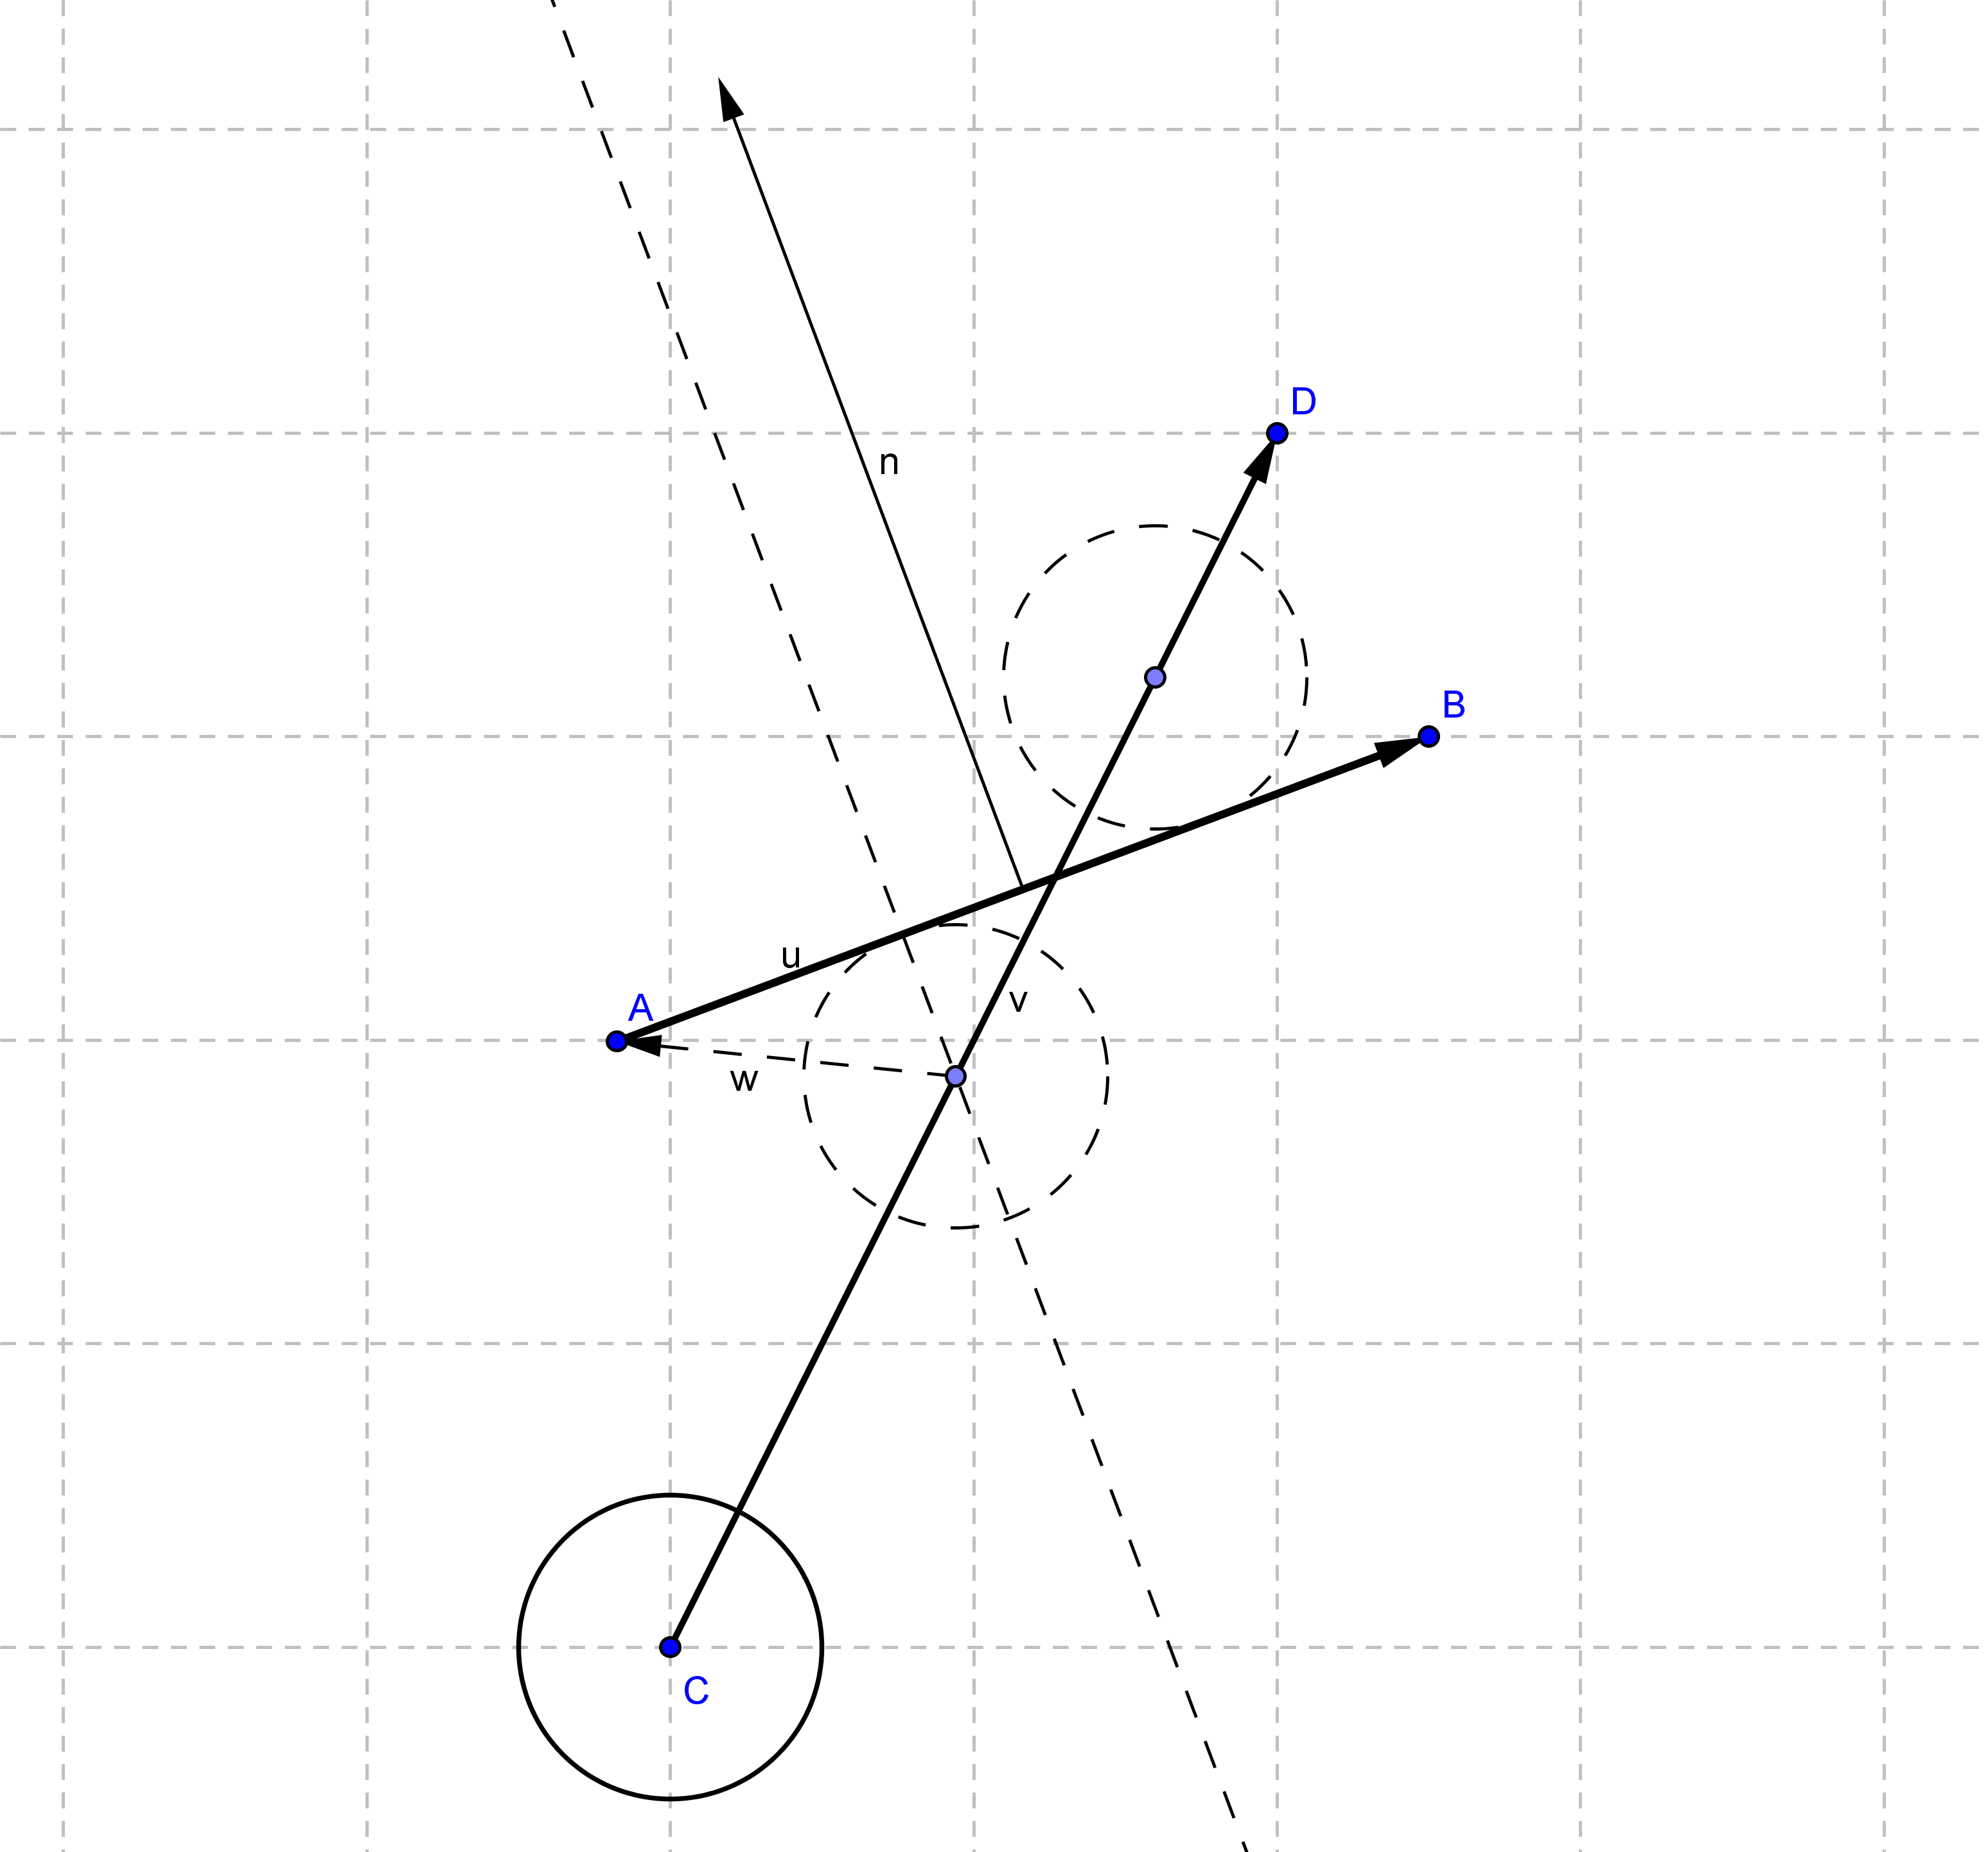
\includegraphics[width=\textwidth]{Plaatjes/Bal-Lijn.png}}
		\caption{Botsing tussen een bal en een lijnstuk}
		\label{bal-lijn}
	\end{figure}
	
	Eerst defini\"{e}ren we $\mathbf{n}$ als de normaalvector van $AB$. Daarna vinden we de afstand van een punt tot een lijnstuk door middel van de eigenschappen van het inproduct van twee vectoren, zoals in vergelijking \eqref{inproduct-cosinus}:
	\begin{equation}
		\label{eigenschappeninproduct}
		cos \gamma = \frac{|\mathbf{w} \cdot \mathbf{n}|}{\| \mathbf{w} \| \| \mathbf{n} \|}
	\end{equation}
	Verder geldt in het driehoekje met zijden $\mathbf{w}$ en $r$:
	\begin{equation}
		\label{driehoekmetzijdew}
		cos \gamma = \frac{r}{\| \mathbf{w}\| }
	\end{equation}
	Samenvoeging van \eqref{eigenschappeninproduct} en \eqref{driehoekmetzijdew} geeft:
	\begin{equation}
		\label{definitiestraal}
		\begin{aligned}
			\frac{r}{\| \mathbf{w}\| } &= \frac{|\mathbf{w} \cdot \mathbf{n}|}{\| \mathbf{w} \| \| \mathbf{n} \|} \\
			r &= \frac{|\mathbf{w} \cdot \mathbf{n}|}{\| \mathbf{n} \|} \\
			r \, \| \mathbf{n} \| &= |\mathbf{w} \cdot \mathbf{n}| \\
			\pm \, r \, \| \mathbf{n} \| &= \mathbf{w} \cdot \mathbf{n}
		\end{aligned}
	\end{equation}
	Vector $\mathbf{w}$ begint in het middelpunt van de cirkel op $CD$ en gaat naar punt $A$, en is dus als volgt de defini\"{e}ren:
	\begin{equation}
		\label{definitiew}
		\begin{aligned}
			\mathbf{w} &= \mathbf{a} - (\mathbf{c} + t \left(\mathbf{d} - \mathbf{c} \right)) \qquad 0 \leq t \leq 1 \\
			&= \mathbf{a} - \mathbf{c} - t \left(\mathbf{d} - \mathbf{c} \right)
		\end{aligned}
	\end{equation}
	Als je $t=0$ invult krijg je $\mathbf{w} = \mathbf{a} - \mathbf{c}$ en als je $t=1$ invult krijg je $\mathbf{w} = \mathbf{a} - \mathbf{d}$.
	
	Nu kun je \eqref{definitiew} invullen in \eqref{definitiestraal} en kun je $t$ uitdrukken in andere variabelen:
	\begin{equation}
		\begin{aligned}
			\pm \, r \, \| \mathbf{n} \| &= (\mathbf{a} - \mathbf{c} - t \left(\mathbf{d} - \mathbf{c} \right)) \cdot \mathbf{n} \\
			\pm \, r \, \| \mathbf{n} \| &= (\mathbf{a} - \mathbf{c}) \cdot \mathbf{n} - t \left(\mathbf{d} - \mathbf{c} \right) \cdot \mathbf{n} \\
			t \left(\mathbf{d} - \mathbf{c} \right) \cdot \mathbf{n} &= \pm \, r \, \| \mathbf{n} \| + (\mathbf{a} - \mathbf{c}) \cdot \mathbf{n} \\
			t &= \frac{\pm \, r \, \| \mathbf{n} \| + (\mathbf{a} - \mathbf{c}) \cdot \mathbf{n}}{\left(\mathbf{d} - \mathbf{c} \right) \cdot \mathbf{n}}
		\end{aligned}
	\end{equation}
	
	En inderdaad geeft deze formule door het plusminusteken twee oplossingen, tenzij de noemer $0$ is, wat betekent dat het lijnstuk en de verplaatsingsvector evenwijdig lopen.
	
	Er is echter nog \'{e}\'{e}n probleem dat we moeten oplossen. Aangezien de formule twee oplossingen geeft voor elke situatie waarbij de verplaatsingsvector en het lijnstuk niet parallel lopen, geeft de formule blijkbaar ook twee oplossingen voor de momenten waarop de cirkel tegen de lijn in het verlengde van het lijnstuk botst. Er moet dus nog gecontroleerd worden of de cirkel wel daadwerkelijk het lijnstuk raakt, of juist de lijn in het verlengde van het lijnstuk.
	
	\subsubsection{Lijnstuk of lijn?}
	De formule uit de vorige paragraaf blijkt dus ook oplossingen te geven voor botsingen met de lijn in het verlengde van het lijnstuk. Om te controleren of er wel sprake is van een botsing met een lijnstuk, kijken we wat de verhouding is tussen het beginpunt van het lijnstuk en het raakpunt van de cirkel en het lijnstuk zelf.
	
	We noemen het middelpunt van de cirkel punt $M$, het raakpunt van de cirkel met lijn $AB$ punt $P$, we stellen het lijnstuk voor als vector $\mathbf{u}$ en we spiegelen vector $\mathbf{w}$. Zie figuur \ref{botsing-lijnstuk-closeup}. Het gaat nu om de verhouding $AP:AB$. Is die verhouding kleiner dan 0 of groter dan 1, dan raakt de cirkel aan de lijn voorbij het lijnstuk. Ligt de verhouding tussen 0 en 1 in, dan raakt de cirkel aan het lijnstuk.

	\begin{figure}[h]
		\centerline{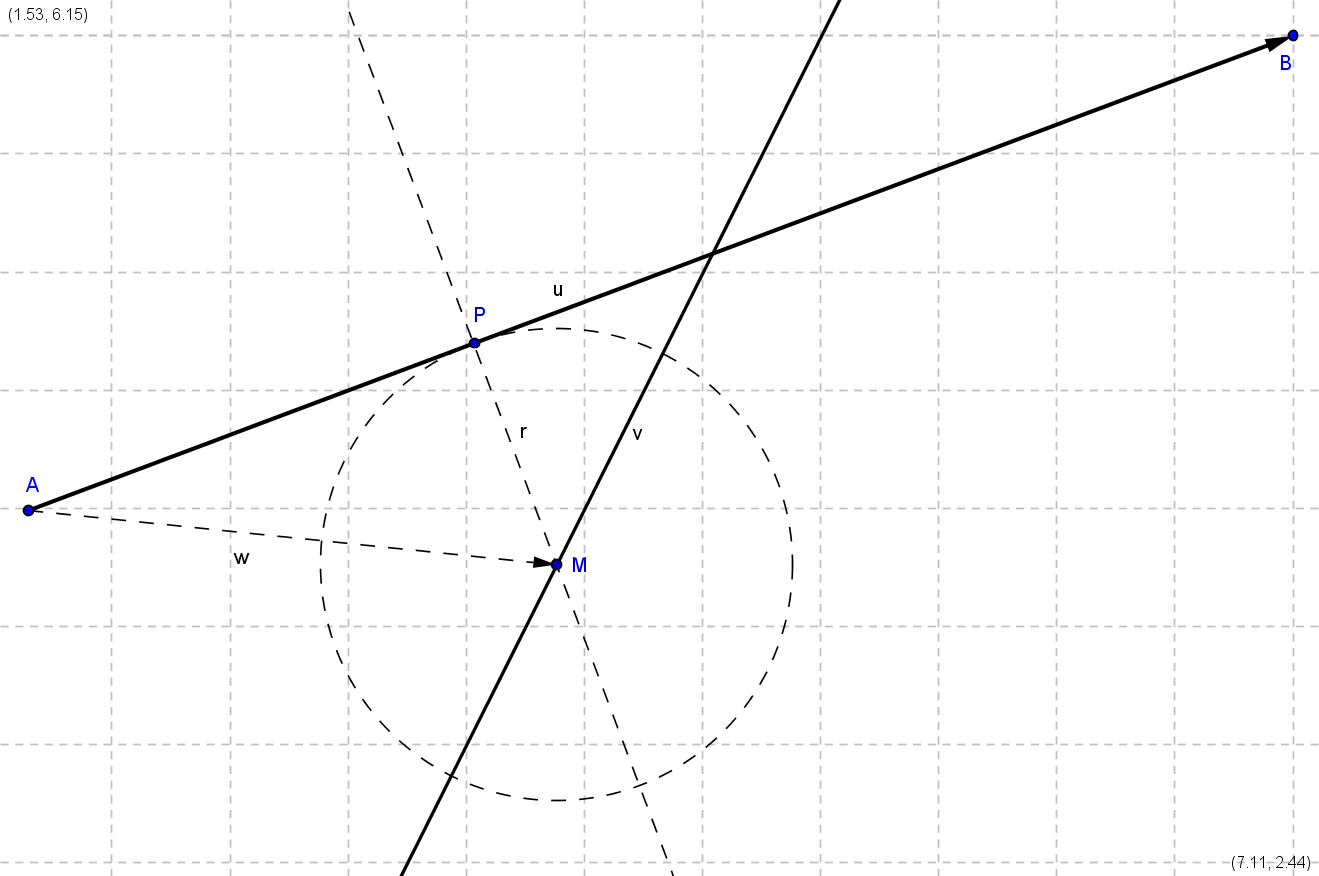
\includegraphics[width=\textwidth]{Plaatjes/Bal-Lijn-stuk-closup.png}}
		\caption{Botsing van een cirkel met een lijnstuk}
		\label{botsing-lijnstuk-closeup}
	\end{figure}	
	
	Eerder \eqref{inproduct-cosinus} bleek al dat geldt:
	\begin{equation}
		\label{inproduct-cosinus-toegepast}
		\begin{aligned}
			\mathbf{u} \cdot \mathbf{w} &= \|\mathbf{u}\| \cdot \|\mathbf{w}\| \cdot \cos\gamma \\
			\cos\gamma &= \frac{\mathbf{u} \cdot \mathbf{w}}{\|\mathbf{u}\| \cdot \|\mathbf{w}\|}\\
		\end{aligned}
	\end{equation}
	\\Verder geldt in driehoek $\triangle AMP$:
	\begin{equation}
		\label{cos-gamma}
		\cos\gamma = \frac{AP}{\|\mathbf{w}\|}
	\end{equation}

	Combineer je \eqref{inproduct-cosinus-toegepast} en \eqref{cos-gamma}, dan krijg je:
	\begin{equation}
		\begin{aligned}
		\frac{AP}{\|\mathbf{w}\|} &= \frac{\mathbf{v} \cdot \mathbf{w}}{\|\mathbf{v}\| \cdot \|\mathbf{w}\|} \\
		                       AP &= \frac{\mathbf{v} \cdot \mathbf{w}}{\|\mathbf{v}\|} \\
		\frac{AP}{\|\mathbf{v}\|} &= \frac{\mathbf{v} \cdot \mathbf{w}}{\|\mathbf{v}\| \cdot \|\mathbf{v}\|} \\
		\frac{AP}{\|\mathbf{v}\|} &= \frac{\mathbf{v} \cdot \mathbf{w}}{\mathbf{v} \cdot \mathbf{v}}\\
		\frac{AP}{AB} &= \frac{\mathbf{v} \cdot \mathbf{w}}{\mathbf{v} \cdot \mathbf{v}}\\
		\end{aligned}
	\end{equation}
	\\We hebben dit ook in \href{http://www.geogebra.org/webstart/geogebra.html}{Geogebra} gesimuleerd, zie in de bijlage het bestand Bal-Lijn.ggb. Variabelen hierbij zijn de positie van de cirkel en de positie van het lijnstuk.
	
	\subsubsection{Uiteinden van het lijnstuk}
	De vergelijking werkt niet om te kijken of een cirkel op \'{e}\'{e}n van de uiteinden van een lijnstuk botst, zoals in figuur \ref{botsing-lijnstuk-uiteinden}. Gelukkig is de oplossing hiervoor heel simpel; de uiteinden van een lijnstuk zijn te zien als een cirkel met straal 0. En omdat we al formules hebben voor botsingen tussen twee cirkels, hebben we geen extra werk.
	
	\begin{figure}[h]
		\centerline{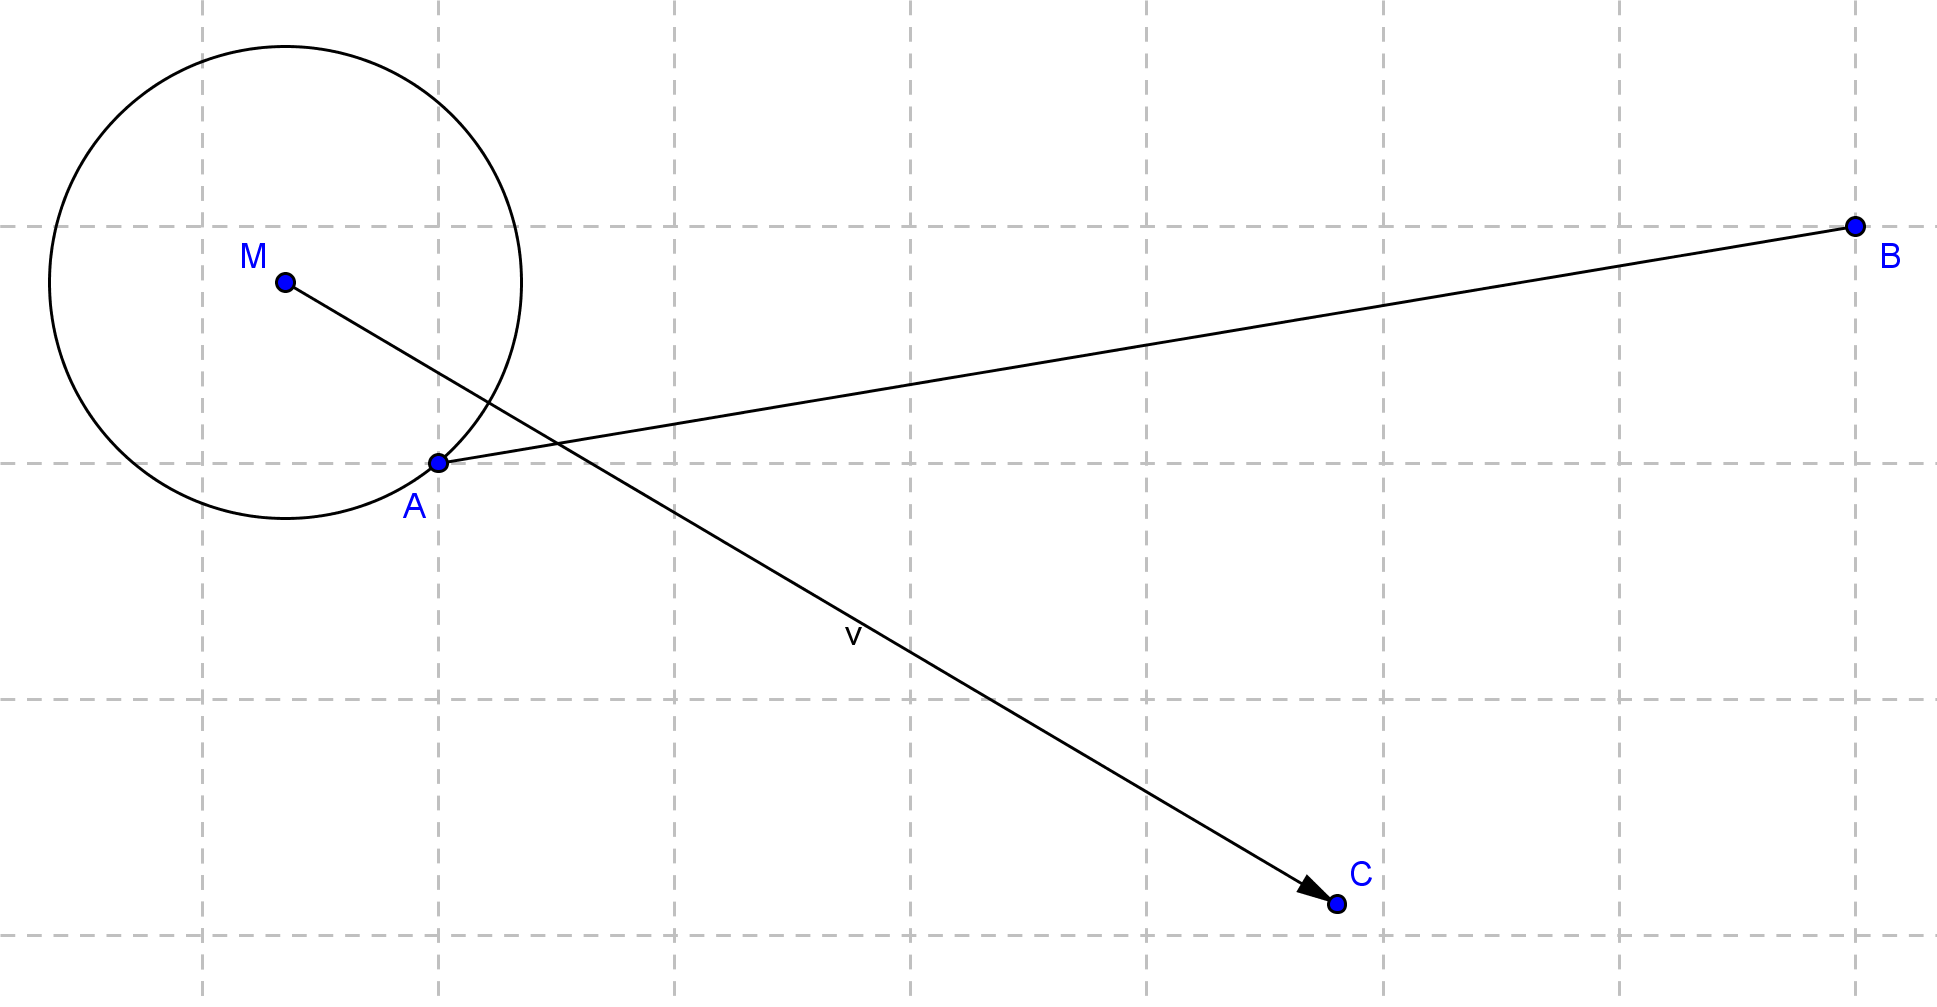
\includegraphics[width=\textwidth]{Plaatjes/Bal-Lijnstuk-Uiteinde.png}}
		\caption{Een cirkel botst tegen het uiteinde van een lijnstuk}
		\label{botsing-lijnstuk-uiteinden}
	\end{figure}
	
	\newpage

	\section{Theorie van botsingen}
	In de natuurkunde is een botsing elke interactie tussen deeltjes of voorwerpen die dicht genoeg bij elkaar komen om energie uit te wisselen. Bij een botsing tussen twee lichamen (voorwerpen) zullen er van het moment van eerste aanraking af vormveranderingen optreden, waardoor veerkrachten worden opgewekt. Als deze veerkrachten groot genoeg zijn, zullen de lichamen zich na de botsing weer van elkaar verwijderen. In het algemeen zijn de snelheden van beide lichamen voor en na de botsing verschillend, zodat overdracht van kinetische energie (bewegingsenergie) heeft plaatsgevonden.

	\subsection{Elastische botsing}
	Als twee biljartballen met elkaar botsen, treedt er slechts een tijdelijke vormverandering op; aan het eind van de botsing krijgen de ballen hun oude vorm weer terug. Dit heet dan van een volkomen elastische (veerkrachtige) botsing, waarvoor de wet van behoud van bewegingsenergie geldig is.

	\subsection{Onelastische botsing}
	Wordt er bijvoorbeeld een kogel in een zandzak geschoten en blijft de kogel daarin steken, dan bewegen beide lichamen zich als \'{e}\'{e}n geheel verder. Bij deze volkomen onelastische botsing treedt een blijvende vormverandering op, zodat de wet van behoud van bewegingsenergie niet geldig is, omdat een deel van de bewegingsenergie verbruikt is voor deze vervorming.
	Tussen deze twee voorbeelden in liggen gedeeltelijke veerkrachtige botsingen.

	\subsection{De wet van behoud van impuls}
	Omdat voor elke botsing geldt dat de krachten die de lichamen op elkaar uitoefenen, even groot zijn, tegengesteld gericht zijn en even lang werken, is de stoot van de botsingskrachten nul:
	\begin{equation}
		  \int_0^t \sum F_i\,dt = 0\\
	\end{equation}

	De verandering van de impuls van de beide lichamen samen is dus nul, met andere woorden: voor elk type botsing geldt de wet van behoud van impuls.
	Voor de gevolgen van een botsing is het ook belangrijk hoe de twee lichamen elkaar treffen. Als je aanneemt dat de beide lichamen in \'{e}\'{e}n plat vlak bewegen, dan kunnen de beide snelheidsvectoren samenvallen met de verbindingslijn tussen de beide zwaartepunten. Dit heet een centrale botsing (analoog met een frontale botsing tussen auto's). Maken deze vectoren hoeken met deze verbindingslijn, dan spreekt men van een niet-centrale botsing (bijvoorbeeld een botsing tussen twee auto's op een straathoek).
	
	\newpage
	
	\section{Berekening van de snelheden na de botsing}
	In de meeste gevallen zijn de snelheden van de ballen na de botsing, anders dan de snelheden van de ballen voor de botsing. Deze snelheden kunnen berekend worden met behulp van de snelheden v\'{o}\'{o}r de botsing en de massa's van beide ballen. Een eenvoudige botsing is de centrale botsing, ook wel eendimensionale botsing genoemd.

	\subsection{Berekening voor een centrale botsing}
	De snelheden na een botsing bij een centrale botsing kunnen op meerdere manieren berekend worden. Hier volgen twee methodes waarop deze berekend kunnen worden. Bij  de eerste methode wordt gebruikt gemaakt van de wet van behoud van energie en de wet van behoud van impuls. Bij de tweede methode wordt alleen de wet van behoud van impuls en de gemeenschappelijke snelheid gebruikt.

	\subsubsection{Met behulp van de wet van behoud van energie en impuls}
	Omdat we te maken hebben met volkomen elastische botsingen geldt de wet van behoud van energie \eqref{energie} en de wet van behoud van impuls \eqref{impuls}. Met deze twee wetten kunnen we de snelheden van de ballen na de botsing berekenen.
	\begin{equation}
		\label{energie}
		\frac{1}{2} m_1 {o_1}^2 + \frac{1}{2} m_2 {o_2}^2 = \frac{1}{2} m_1{v_1}^2 + \frac{1}{2}m_2 {v_2}^2\\
	\end{equation}
	\begin{equation}
		\label{impuls}
		m_1 o_1 + m_2 o_2 =  m_1 v_1 + m_2 v_2\\
	\end{equation}
	\\Waarbij:
	\begin{equation}
		\begin{aligned}
			m_1 &= \text{massa van lichaam 1}\\
			m_2 &= \text{massa van lichaam 2}\\
			o_1 &= \text{snelheid van lichaam 1 voor de botsing}\\
			o_2 &= \text{snelheid van lichaam 2 voor de botsing}\\
			v_1 &= \text{snelheid van lichaam 1 na de botsing}\\
			v_2 &= \text{snelheid van lichaam 2 na de botsing}\\
		\end{aligned}
	\end{equation}

	We hebben nu twee vergelijkingen met twee onbekenden, namelijk $v_1$ en $v_2$. We kunnen $v_2$ uit beide vergelijkingen elimineren, en daarna de vergelijkingen aan elkaar gelijk stellen, zodat we als onbekende alleen $v_1$ over houden.
	\\Als eerste de vergelijking van de wet van behoud van energie:
	\begin{equation}
		\label{energie-{v_1}^2}
		\begin{aligned}
			\frac{1}{2} m_1 {o_1}^2 + \frac{1}{2} m_2 {o_2}^2 &= \frac{1}{2} m_1{v_1}^2 + \frac{1}{2}m_2 {v_2}^2\\
			m_1 {o_1}^2 + m_2 {o_2}^2 &= m_1{v_1}^2 + m_2 {v_2}^2\\
			m_1 {o_1}^2 + m_2 {o_2}^2 - m_2 {v_1}^2 &= m_2{v_2}^2\\
			\frac{m_1 {o_1}^2 + m_2 {o_2}^2 - m_1 {v_1}^2}{m_2} &= {v_2}^2\\
		\end{aligned}
	\end{equation}
	\\Dan de vergelijking van de wet van behoud van impuls:
	\begin{equation}
		\label{impuls-{v_1}^2}
		\begin{aligned}
			m_1 o_1 + m_2 o_2 &=  m_1 v_1 + m_2 v_2\\
			m_1 o_1 + m_2 o_2 - m_1 v_1 &=  m_2 v_2\\
			\frac{m_1 o_1 + m_2 o_2 - m_1 v_1}{m_2} &= v_2\\
			{\left(\frac{m_1 o_1 + m_2 o_2 - m_1 v_1}{m_2}\right)}^2 &= {v_2}^2\\
		\end{aligned}
	\end{equation}
	\\De uitkomsten van \eqref{impuls-{v_1}^2} en \eqref{energie-{v_1}^2} aan elkaar gelijk stellen geeft:
	\begin{equation}
		\begin{aligned}
			&\frac{m_1 {o_1}^2 + m_2 {o_2}^2 - m_1 {v_1}^2}{m_2} = {\left(\frac{m_1 o_1 + m_2 o_2 - m_1 v_1}{m_2}\right)}^2\\
			&= \frac{\left({m_1}^2{o_1}^2 + {m_2}^2{o_2}^2 + {m_1}^2{v_1}^2\right) + \left(2m_1m_2o_1o_2 - 2{m_1}^2o_1v_1 - 2m_1m_2o_2v_1\right)}{{m_2}^2}\\
		\end{aligned}
	\end{equation}
	\\Deze vergelijking oplossen, zodat je een vierkantsvergelijking krijgt:
	\begin{equation}
		\begin{aligned}
			&{m_1}^2{o_1}^2 + {m_2}^2{o_2}^2 + {m_1}^2{v_1}^2 + 2m_1m_2o_1o_2 - 2{m_1}^2o_1v_1 - 2m_1m_2o_2v_1 =\\
			&m_1m_2{o_1}^2 + {m_2}^2{o_2}^2 - m_1m_2{v_1}^2\\
			&{m_1}^2{o_1}^2 + {m_1}^2{v_1}^2 + 2m_1m_2o_1o_2 - 2{m_1}^2o_1v_1 - 2m_1m_2o_2v_1 =\\
			&m_1m_2{o_1}^2 - m_1m_2{v_1}^2\\
			&{m_1}^2{o_1}^2 + {m_1}^2{v_1}^2 + 2m_1m_2o_1o_2 - 2{m_1}^2o_1v_1 - 2m_1m_2o_2v_1 - m_1m_2{o_1}^2 + m_1m_2{v_1}^2 = 0\\
			&\left({m_1}^2+m_1m_2\right){v_1}^2+\left(-2{m_1}^2o_1-2m_1m_2o_2\right)v_1+\left({m_1}^2{o_1}^2+2m_1m_2o_1o_2-m_1m_2{o_1}^2\right) = 0\\
		\end{aligned}
	\end{equation}
	\\De oplossingen worden gegeven door: $v_1=\frac{-b\pm\sqrt{b^2-4ac}}{2a}$, waarbij:
	\begin{equation}
		\begin{aligned}
			a &= {m_1}^2+m_1m_2\\
			b &= -2{m_1}^2o_1-2m_1m_2o_2\\
			c &= {m_1}^2{o_1}^2+2m_1m_2o_1o_2-m_1m_2{o_1}^2\\
		\end{aligned}
	\end{equation}
	\\We berekenen $-b$, $b^2$, $4ac$ en $b^2-4ac$ apart:
	\begin{equation}
		\begin{aligned}
			-b&=-\left(-2{m_1}^2o_1-2m_1m_2o_2\right)\\
			&=2{m_1}^2o_1+2m_1m_2o_2\\
		\end{aligned}
	\end{equation}

	\begin{equation}
		\begin{aligned}
			b^2&=\left(-2{m_1}^2o_1-2m_1m_2o_2\right)^2\\
			&=4{m_1}^4{o_1}^2+8{m_1}^3m_2o_1o_2+4{m_1}^2{m_2}^2{o_2}^2\\
		\end{aligned}
	\end{equation}

	\begin{equation}
		\begin{aligned}
			4ac&=4\left({m_1}^2+m_1m_2\right)\left({m_1}^2{o_1}^2+2m_1m_2o_1o_2-m_1m_2{o_1}^2\right)\\
			&=4{m_1}^4{o_1}^2+8{m_1}^3m_2o_1o_2+8{m_1}^2{m_2}^2o_1o_2-4{m_1}^2{m_2}^2{o_1}^2\\
		\end{aligned}
	\end{equation}

	\begin{equation}
		\begin{aligned}
				b^2-4ac&=4{m_1}^4{o_1}^2+8{m_1}^3m_2o_1o_2+4{m_1}^2{m_2}^2{o_2}^2-4\left({m_1}^2+m_1m_2\right)*\\
			&\left({m_1}^2{o_1}^2+2m_1m_2o_1o_2-m_1m_2{o_1}^2\right)\\
			&={m_1}^2{m_2}^2{\left(2o_2-2o_1\right)}^2\\
		\end{aligned}
	\end{equation}
	\\De vierkantsvergelijking kan nu worden ingevuld:
	\begin{equation}
		\begin{aligned}
			v_1&=\frac{-b\pm\sqrt{b^2-4ac}}{2a}\\
			&=\frac{\left(2{m_1}^2o_1+2m_1m_2o_2\right)\pm\sqrt{{m_1}^2{m_2}^2{\left(2o_2-2o_1\right)}^2}}{2\left({m_1}^2+m_1m_2\right)}\\
			&=\frac{\left(m_1o_1+m_2o_2\right)+m_2\left(o_2-o_1\right)}{\left(m_1+m_2\right)}\\
		\end{aligned}
	\end{equation}
	\\Je kunt $v_2$ op dezelfde manier berekenen. Dus $v_1$ en $v_2$ zijn:
	\begin{equation}
		\begin{aligned}
		\label{uitwerking-energie-impuls}
			v_1&=\frac{\left(m_1o_1+m_2o_2\right)+m_2\left(o_2-o_1\right)}{\left(m_1+m_2\right)} \wedge v_2&=\frac{\left(m_2o_2+m_1o_1\right)+m_1\left(o_1-o_2\right)}{\left(m_2+m_1\right)}\\
		\end{aligned}
	\end{equation}

	\subsubsection{Met behulp van de gemeenschappelijke snelheid}
	Net zoals bij de vorige manier gebruiken we de wet van behoud van impuls \eqref{impuls-{v_1}^2}, omdat bij botsingen alleen onderlinge krachten werken. We defini\"{e}ren $v_g$ als de gemeenschappelijke snelheid  aan het eind van de eerste periode van de centrale botsing. Dan geldt er:
	\begin{equation}
		\begin{aligned}
			m_1o_1+m_2o_2&=m_1v_g+m_2v_g\\
		\end{aligned}
	\end{equation}
	\\Waarbij:
	\begin{equation}
		\begin{aligned}
			m_1 &= \text{massa van lichaam 1}\\
			m_2 &= \text{massa van lichaam 2}\\
			o_1 &= \text{snelheid van lichaam 1 voor de botsing}\\
			o_2 &= \text{snelheid van lichaam 2 voor de botsing}\\
		\end{aligned}
	\end{equation}
	\\Daaruit volgt:
	\begin{equation}
		\begin{aligned}
		\label{gemeenschappelijke-snelheid}
			v_g&=\frac{m_1o_1+m_2o_2}{m_1+m_2}\\
		\end{aligned}
	\end{equation}
	\\Bij een volkomen onelastische botsing is de gemeenschappelijke snelheid $v_g$ van beide voorwerpen gelijk aan \eqref{gemeenschappelijke-snelheid}. Bij een volkomen elastische centrale botsing is de snelheidsverandering van elk voorwerp gedurende de tweede periode van de botsing (op grond van de definitie van een elastische botsing) gelijk aan de snelheidsverandering gedurende de eerste periode van de botsing.
	Is $v$ de snelheid na de botsing, dan geldt dus:
	\begin{equation}
		\begin{aligned}
			v-v_g&=v_g-o\\
			v&=2v_g-o\\
		\end{aligned}
	\end{equation}
	\\Voor de snelheden $v_1$ en $v_2$ van de twee voorwerpen na de botsing geldt dus:
	\begin{equation}
		\begin{aligned}
		\label{snelheden-met-gemeenschappelijke-snelheid}
			v_1&=v_g+(v_g-o_1)=2v_g-o_1\\
			v_2&=v_g+(v_g-o_2)=2v_g-o_2\\
		\end{aligned}
	\end{equation}
	\\Wanneer we \eqref{gemeenschappelijke-snelheid} substitueren in \eqref{snelheden-met-gemeenschappelijke-snelheid} krijgen we de volgende vergelijkingen:
	\begin{equation}
		\begin{aligned}
		\label{uitwerking-gemeenschappelijke-snelheid}
			v_1=2\left(\frac{m_1o_1+m_2o_2}{m_1+m_2}\right)-o_1 &\wedge v_2=2\left(\frac{m_1o_1+m_2o_2}{m_1+m_2}\right)-o_2\\
			v_1=\frac{2\left(m_1o_1+m_2o_2\right)}{m_1+m_2}-v_1\cdot\frac{m_1+m_2}{m_1+m_2} &\wedge v_2=\frac{2\left(m_1o_1+m_2o_2\right)}{m_1+m_2}-v_2\cdot\frac{m_1+m_2}{m_1+m_2}\\
			v_1=\frac{2\left(m_1o_1+m_2o_2\right)-v_1\left(m_1+m_2\right)}{m_1+m_2} &\wedge v_2=\frac{2\left(m_1o_1+m_2o_2\right)-v_2\left(m_1+m_2\right)}{m_1+m_2}\\
			v_1=\frac{2m_1o_1+2m_2o_2-m_1o_1-m_2o_1}{m_1+m_2} &\wedge v_2=\frac{2m_1o_1+2m_2o_2-m_1o_2-m_2o_2}{m_1+m_2}\\
			v_1=\frac{m_1o_1+2m_2o_2-o_1m_2}{m_1+m_2} &\wedge v_2=\frac{2m_1o_1+m_2o_2-o_2m_1}{m_1+m_2}\\
			v_1=\frac{m_1o_1+m_2o_2+m_2o_2-o_1m_2}{m_1+m_2} &\wedge v_2=\frac{m_1o_1+m_2o_2+m_1o_1-o_2m_1}{m_1+m_2}\\
			v_1=\frac{\left(m_1o_1+m_2o_2\right)+m_2\left(o_2-o_1\right)}{m_1+m_2} &\wedge v_2=\frac{\left(m_1o_1+m_2o_2\right)+m_1\left(o_1-o_2\right)}{m_1+m_2}\\
		\end{aligned}
	\end{equation}
	\\De uitkomst van \eqref{uitwerking-gemeenschappelijke-snelheid} komt overeen met de uitkomst van \eqref{uitwerking-energie-impuls}. De formule voor de snelheden na de botsing is dus als volgt:

	\begin{equation}
		\label{snelheden-na-botsing}
			\boxed{v_1=\frac{\left(m_1o_1+m_2o_2\right)+m_2\left(o_2-o_1\right)}{m_1+m_2} \wedge v_2=\frac{\left(m_1o_1+m_2o_2\right)+m_1\left(o_1-o_2\right)}{m_1+m_2}}
	\end{equation}

	\subsection{Berekening voor een niet-centrale botsing}
	Je kunt de bovenstaande vergelijkingen niet toepassen op niet-centrale botsingen, omdat je niet weet onder welke hoek ze elkaar raken. Alleen de snelheden en de massa zijn gebruikt in de formules, en er is dus niets gegeven over de posities en de richting van de snelheid, en dat is nu net wat nodig is voor het berekenen van allerlei soorten botsingen. De volgende gegevens hebben we nodig als we de snelheden na een niet-centrale botsing willen berekenen:
	\begin{equation}
		\begin{aligned}
			x_1 &= \text{x-positie van lichaam 1}\\
			y_1 &= \text{y-positie van lichaam 1}\\
			x_2 &= \text{x-positie van lichaam 2}\\
			y_2 &= \text{y-positie van lichaam 2}\\
			o_{1,x} &= \text{snelheid in de x-richting van lichaam 1 voor de botsing}\\
			o_{1,y} &= \text{snelheid in de y-richting van lichaam 1 voor de botsing}\\
			o_{2,x} &= \text{snelheid in de x-richting van lichaam 2 voor de botsing}\\
			o_{2,y} &= \text{snelheid in de y-richting van lichaam 2 voor de botsing}\\
		\end{aligned}
	\end{equation}
	Bij een centrale botsing bewegen de twee lichamen langs de verbindingslijn van de middelpunten. De botsing vindt ook plaats langs deze lijn, het wordt daarom ook wel een eendimensionale botsing genoemd. Bij een niet-centrale botsing kunnen de snelheden ook ontbonden worden in snelheden langs de verbindingslijn en snelheden loodrecht op de verbindings lijn. Als er alleen gekeken wordt naar de snelheid langs de verbindingslijn, dan kan daar formule \eqref{snelheden-na-botsing} op worden toegepast omdat het een eendimensionale botsing betreft. De snelheid die loodrecht op deze verbindingslijn staat is onafhankelijk van de botsing, en zal dus constant blijven.

	\begin{figure}[H]
		\centerline{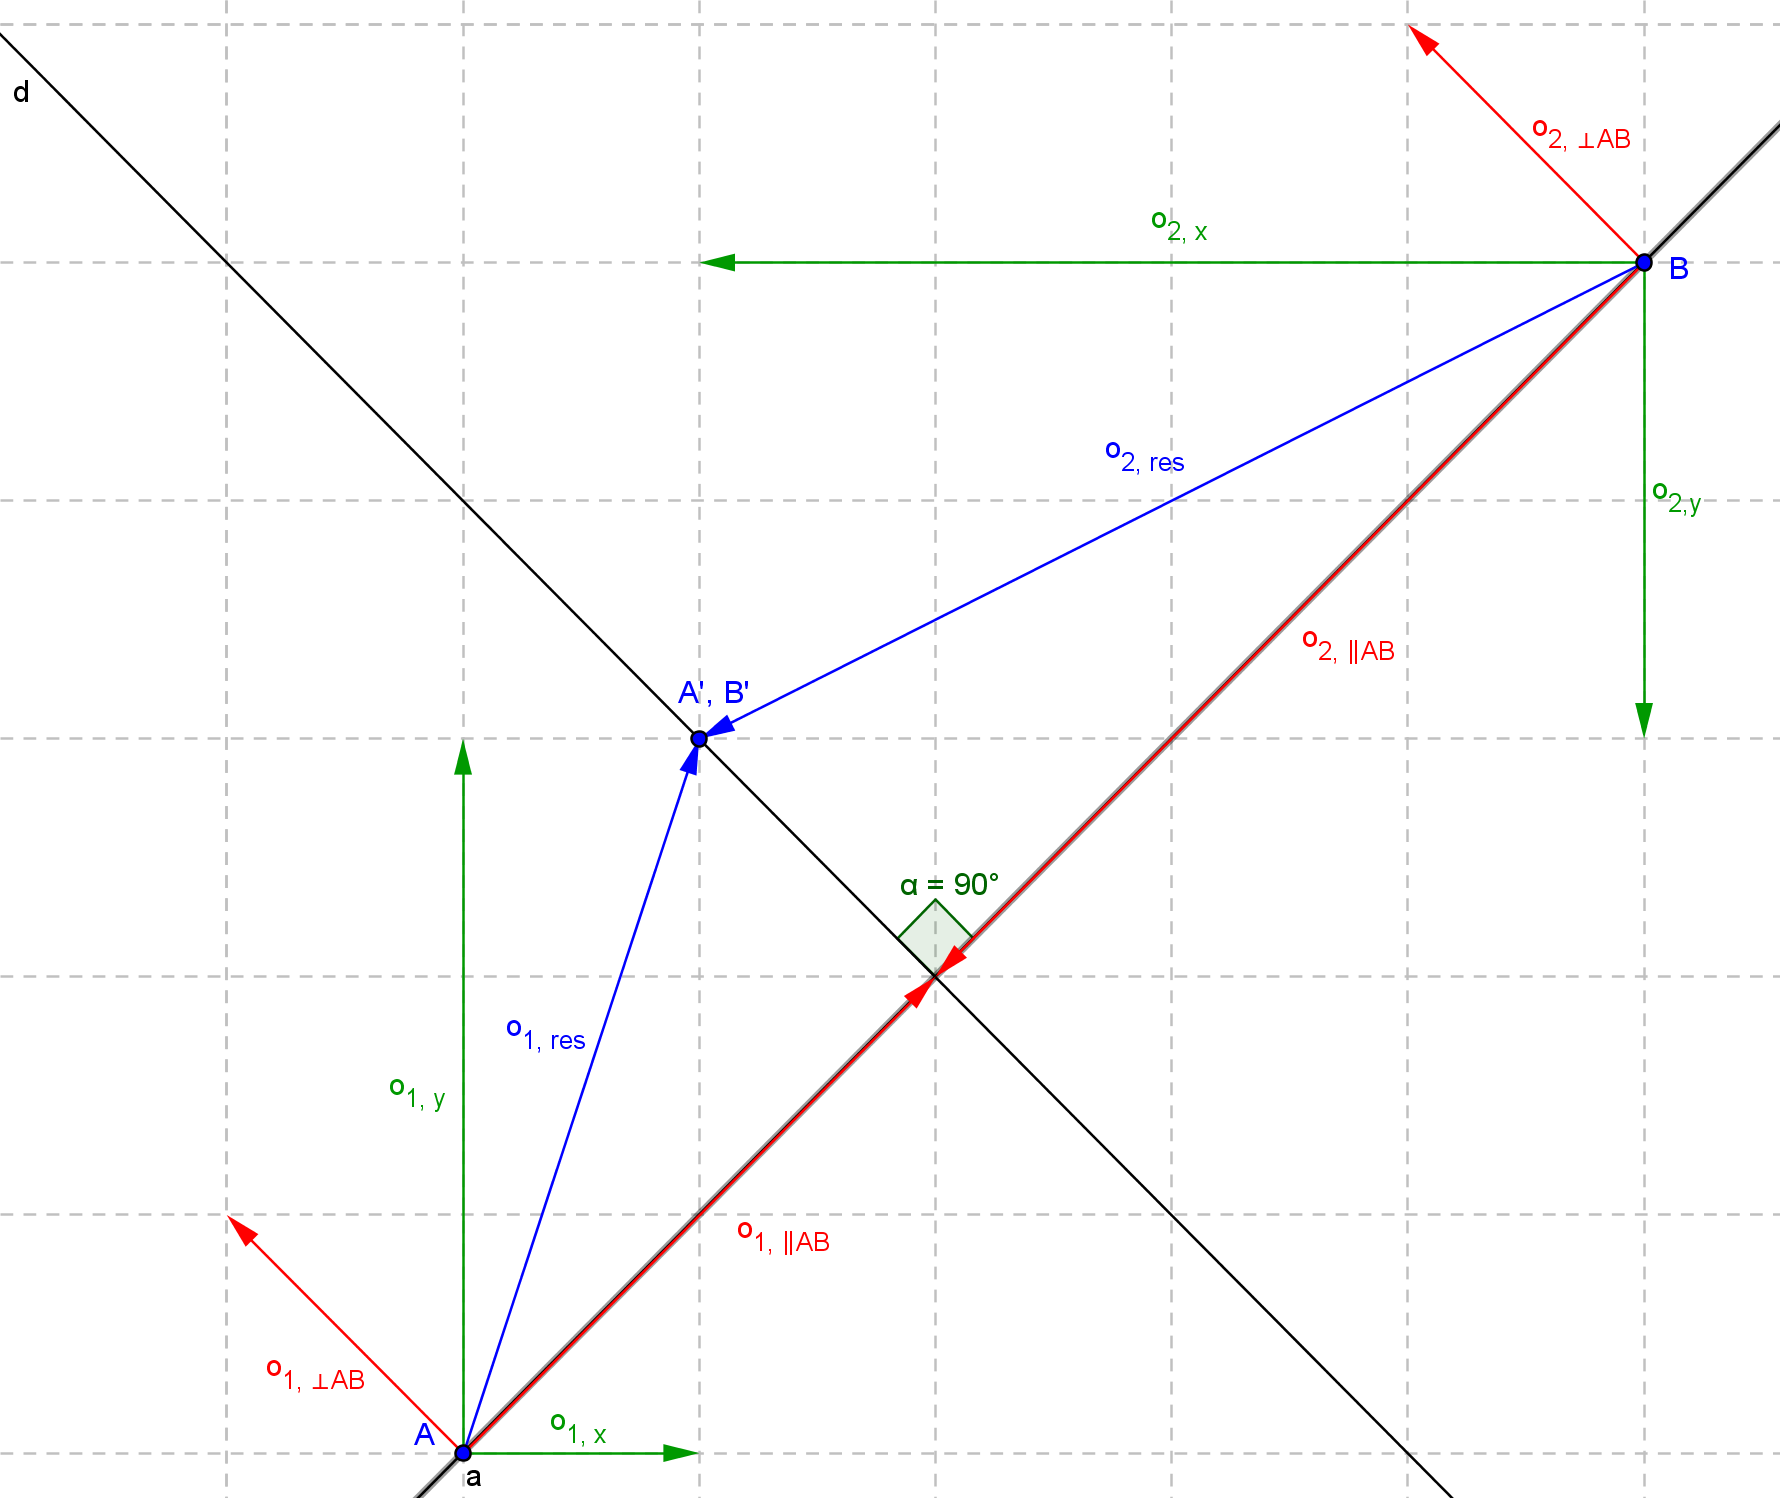
\includegraphics[width=\textwidth]{Plaatjes/niet-centrale-botsing.png}}
		\caption{Botsing tussen twee ballen}
		\label{niet-centrale botsing}
	\end{figure}

	De snelheden van lichaam 1 en 2  in de richting van de voortplantingsbeweging zijn:
	\begin{equation}
		\begin{aligned}
			o_1=\sqrt{{o_{1,x}}^2+{{o_{1,y}}^2}}\\
			o_2=\sqrt{{o_{2,x}}^2+{{o_{2,y}}^2}}\\
		\end{aligned}
	\end{equation}

	Als we eerst de vergelijking opstellen voor bal 1, zijn die van bal 2 daar eenvoudig uit te herleiden. De positie van bal 1 is $(x_1,y_1)$. Na $\text{1 }s$ is de positie van bal 1 $(x_1+o_{1,x},y_1+o_{1,y})$. Wanneer een frame een andere lengte heeft dan $\text{1 }s$ moeten de snelheden nog vermenigvuldigd worden met een constante. Voor het gemak geven we de verschillende grootheden een letter:
	\begin{equation}
		\begin{aligned}
			A&=\text{lichaam 1}\\
			B&=\text{lichaam 2}\\
			A'&=\text{lichaam 1 op de positie van de botsing}\\
			B'&=\text{lichaam 2 op de positie van de botsing}\\
			a&={x_1}\\
			b&={y_1}\\
			c&={x_2}\\
			d&={y_2}\\
			e&={x_1+o_{1,x}}={x_2+o_{2,x}}\\
			f&={y_1+o_{1,y}}={y_2+o_{2,y}}\\
		\end{aligned}
	\end{equation}
	We bekijken de tweedimentionale botsing in het $Oxy$-vlak, en lossen het dan analytisch op. Het middelpunt is $M(\frac{x_1+x_2}{2}, \frac{y_1+y_2}{2})$. De vergelijking voor AM en A'M zijn dan als volgt:

	\begin{equation}
		\begin{aligned}
			AM=AB&: y-b=\frac{b-d}{a-c}\left(x-a\right)\\
			A'M&: y-f=\frac{c-a}{b-d}\left(x-e\right)\\
		\end{aligned}
	\end{equation}

	We kunnen het snijpunt van deze twee vergelijkingen berekenen. De $x$-co"{o}rdinaat stelt de snelheid in de $x$-richting naar B voor. De $y$-co\"{o}rdinaat stelt de snelheid in de $y$-richting naar B voor.
	\begin{equation}
		\begin{aligned}
			\frac{b-d}{a-c}\left(x-a\right)+b=&\frac{c-a}{b-d}\left(x-e\right)+f\\
			\left(\frac{b-d}{a-c}+\frac{a-c}{b-d}\right)x=&\frac{b-d}{a-c}a+\frac{a-c}{b-d}e+f-b\\
			\frac{(b-d)^2+(a-c)^2}{(a-c)(b-d)}x=&\frac{a(b-d)^2+e(a-c)^2+(f-b)(a-c)(b-d)}{(a-c)(b-d)}\\
			\left((b-d)^2+(a-c)^2\right)x=&a(b-d)^2+e(a-c)^2+(f-b)(a-c)(b-d)\\
			x=&\frac{a(b-d)^2+e(a-c)^2+(f-b)(a-c)(b-d)}{(b-d)^2+(a-c)^2}\\
		\end{aligned}
	\end{equation}

	Invullen in AB geeft 
	\begin{equation}
		\begin{aligned}
		\label{y}
			y=\frac{b-d}{a-c}\left(\frac{a(b-d)^2+e(a-c)^2+(f-b)(a-c)(b-d)}{(b-d)^2+(a-c)^2}-a\right)+b\\
		\end{aligned}
	\end{equation}
	De snelheid richting B is dus: $o_{1, \parallel AB}=\sqrt{x^2+y^2}$. Hiervoor geldt dus wel de wet van behoud van impuls. Voor de snelheid loodrecht op de verplaatsingsrichting geldt: $o_{1, \perp AB}=v_{1, \perp AB}=\sqrt{{o_{1, res}}^2-{o_{1, \parallel AB}}^2}$.

	De snelheid richting B is dus: $o_{1, \parallel AB}=\sqrt{x^2+y^2}$. Hiervoor geldt dus wel de wet van behoud van impuls. Voor de snelheid loodrecht op de verplaatsingsrichting geldt: $o_{1, \perp AB}=v_{1, \perp AB}=\sqrt{{o_{1, res}}^2-{o_{1, \parallel AB}}^2}$.
	
	De resulterende snelheid na de botsing is: $v_{1, res}=\sqrt{{v_{1, \parallel AB}}^2+{v_{1, \perp AB}}^2}$.

	De snelheden in de $x$- en $y$-richting kunnen als volgt berekend worden:
	\begin{equation}
		\begin{aligned}
			v_{1, x}=\frac{v_{1, \parallel AB}\left(a-c\right)+v_{1, \perp AB}\left(b-d\right)}{\sqrt{\left(a-c\right)^2+\left(b-d\right)^2}}\\
			v_{1, y}=\frac{v_{1,  \parallel AB}\left(b-d\right)+v_{1, \perp AB}\left(a-c\right)}{\sqrt{\left(a-c\right)^2+\left(b-d\right)^2}}\\
		\end{aligned}
	\end{equation}

	Nu $a$, $b$, $c$ en $d$ vervangen door de co\"{o}dinaten:
	\begin{equation}
		\begin{aligned}
			v_{1, x}=\frac{v_{1,  \parallel AB}\left(x_1-x_2\right)+v_{1, \perp AB}\left(y_1-y_2\right)}{\sqrt{\left(x_1-x_2\right)^2+\left(y_1-y_2\right)^2}}\\
			v_{1, y}=\frac{v_{1,  \parallel AB}\left(y_1-y_2\right)+v_{1, \perp AB}\left(x_1-x_2\right)}{\sqrt{\left(x_1-x_2\right)^2+\left(y_1-y_2\right)^2}}\\
		\end{aligned}
	\end{equation}
	
	Met alle bekende variabelen:
	De resulterende snelheid na de botsing is: 
	\begin{equation}
		\begin{aligned}
			v_{1, res}&=\sqrt{{v_{1,  \parallel AB}}^2+{v_{1, \perp AB}}^2}\\
			v_{1, res}&=\sqrt{{v_{1,  \parallel AB}}^2+|{o_{1, res}}^2-{o_{1,  \parallel AB}}^2|}\\
			v_{1, res}&=\sqrt{\frac{\left(m_1o_{1,  \parallel AB}+m_2o_{2,  \parallel AB}\right)+m_2\left(o_{2,  \parallel AB}-o_{1,  \parallel AB}\right)}{m_1+m_2}+|{o_{1, res}}^2-{o_{1,  \parallel AB}}^2|}\\
		\end{aligned}
	\end{equation}

	\newpage

	\section{Experiment van botsende ballen}
	Wij werken alleen met botsingen in het platte vlak. Omdat we werken met jeu de boules-ballen zullen we geen volkomen elastische botsingen hebben, dit is overigens in de praktijk nauwelijks haalbaar.

	\subsection{Verwachtingen bij het experiment van botsende ballen}

	\subsubsection{Botsing tussen twee ballen}
	Er zijn twee soorten botsingen te onderscheiden: een centrale botsing en een niet-centrale botsing. De verwachting bij een centrale botsing tussen twee ballen met dezelfde massa is dat de richting van de snelheid van de ballen na de botsing precies tegenovergesteld is aan de richting van de snelheid van de ballen voor de botsing, en dat de snelheden van de ballen verwisseld zijn.
Bij een niet-centrale botsing tussen twee ballen met dezelfde massa waarvan \'{e}\'{e}n bal geen snelheid heeft, zullen de ballen onder een hoek van $90^{\circ}$ uit elkaar gaan na de botsing. 

	Er zijn twee soorten botsingen te onderscheiden: een centrale botsing en een niet-centrale botsing.

	De verwachting bij een centrale botsing is, dat de richting van de snelheid van de ballen na de botsing precies tegenovergesteld is aan de richting van de snelheid van de ballen voor de botsing, en dat de snelheden van de ballen verwisseld zijn.
	De verwachting bij een niet-centrale botsing waarvan \'{e}\'{e}n bal geen snelheid heeft is, dat de ballen onder een hoek van $90^{\circ}$ uitelkaar gaan na de botsing, als de massa's gelijk zijn. 
	
	\begin{figure}[H]
		\centerline{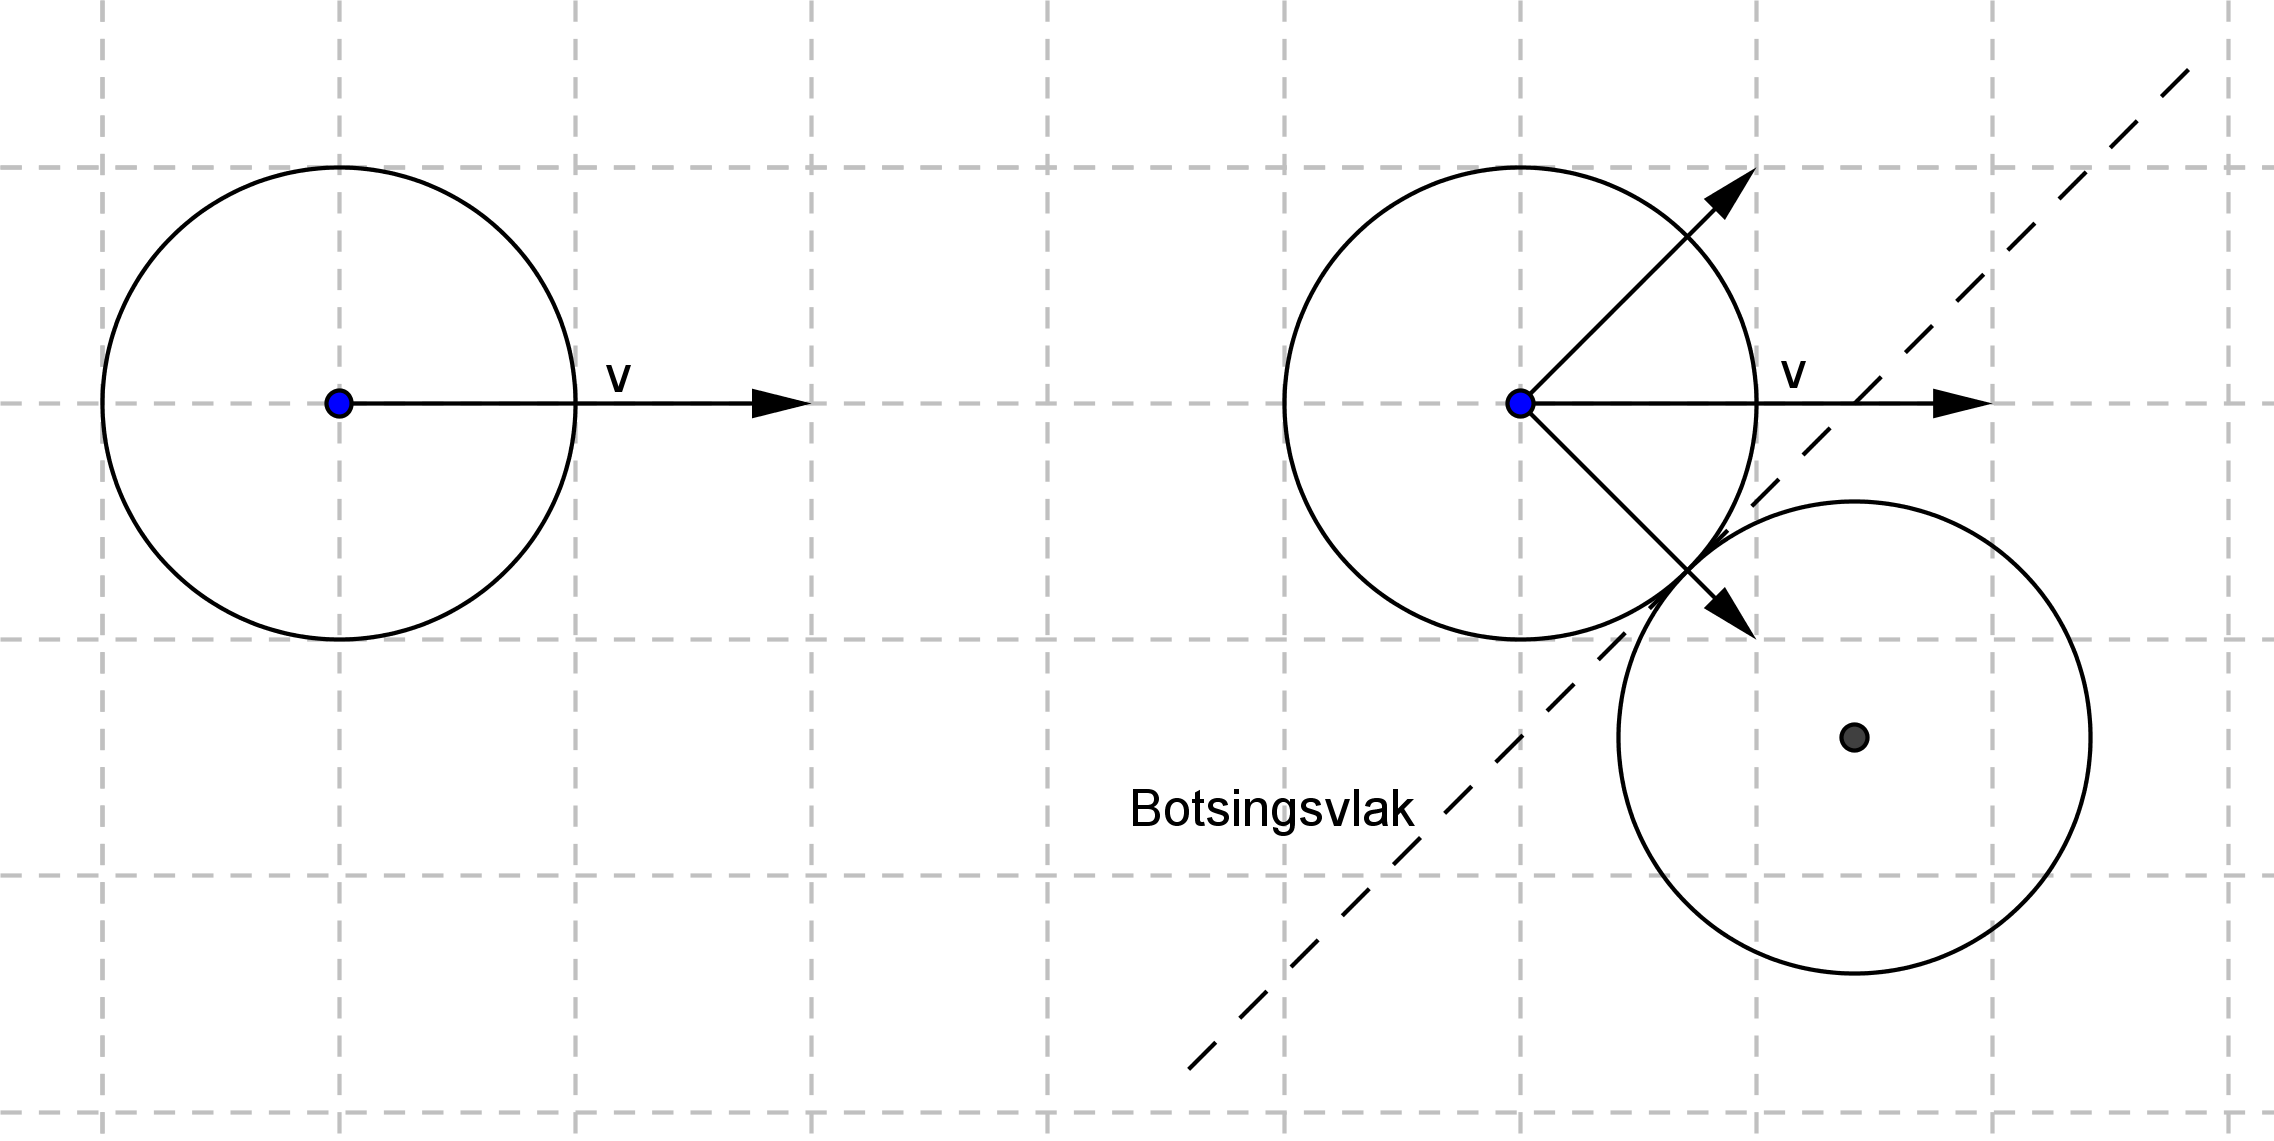
\includegraphics{Plaatjes/BotsingSchuin-2.png}}
		\caption{Een niet-centrale botsing}
		\label{botsingschuin}
	\end{figure}
	
	Op deze twee afbeeldingen heeft bal 2 aanvankelijk geen snelheid. Na de botsing zal een deel van de snelheid van bal 1\ ``overgedragen" zijn aan bal 2, en gaan de ballen onder een hoek van $90^{\circ}$ uit elkaar.

	Dit is ook als volgt te bewijzen:
	De twee ballen zijn te beschouwen als puntmassa's. We kiezen een assenstelsel zo dat er voor de botsing geen beweging in de $y$-richting is. Bal 1 gaat daarna omhoog onder een hoek $\alpha$ en bal 2 onder een hoek $\beta$. Nu hebben we de volgende gegevens:
	\begin{equation}
	\begin{aligned}
		o_{1, x}&=o_1\\
		o_{1, y}&=0\\
		o_{2, x}&=0\\
		o_{2, y}&=0\\
	\end{aligned}
	\end{equation}

	Volgens de wet van behoud van impuls geldt voor de $x$-richting:
	\begin{equation}
	\begin{aligned}
	\label{voorbeeld 1.1}
		mo_{1, x}&=mv_{1, x}+mv_{2, x}\\
		mo_{1, x}&=mv_1cos(\alpha)+mv_2cos(\beta)\\
		{o_{1, x}}^2&={v_1}^2cos^2(\alpha)+{v_2}^2cos^2(\beta)+2v_1v_2cos(\alpha)cos(\beta)\\
	\end{aligned}
	\end{equation}

	En in de $y$-richting geldt:
	\begin{equation}
	\begin{aligned}
	\label{voorbeeld 1.2}
		mo_{1, y}&=mv_{1, y}+mv_{2, y}\\
		0&=mv_{1, y}+mv_{2, y}\\
		0&=mv_1sin(\alpha)+mv_2sin(\beta)\\
	\end{aligned}
	\end{equation}

	Ook geldt de wet van behoud van energie:
	\begin{equation}
	\begin{aligned}
	\label{voorbeeld 1.3}
		m{o_1}^2&=m{v_1}^2+m{v_2}^2\\
		{o_1}^2&={v_1}^2+{v_2}^2\\
	\end{aligned}
	\end{equation}

	Met $sin^2(\alpha)+cos^2(\alpha)=1$ en invullen van \eqref{voorbeeld 1.1} en \eqref{voorbeeld 1.3} in elkaar, levert dat op:
	\begin{equation}
	\begin{aligned}
	\label{voorbeeld 1.4}
		2v_1v_2cos(\alpha)cos(\beta)&={v_1}^2sin^2(\alpha)+{v_2}^2sin^2{\beta}\\
	\end{aligned}
	\end{equation}

	Met gebruik van \eqref{voorbeeld 1.2} in \eqref{voorbeeld 1.4} krijg je dan:
	\begin{equation}
	\begin{aligned}
	\label{voorbeeld 1.5}
		2v_1v_2cos(\alpha)cos(\beta)&=2v_1v_2sin(\alpha)sin(\beta)\\
	\end{aligned}
	\end{equation}

	Dit levert op $tan(\alpha)tan(\beta)=1$ waardoor de hoek $\alpha+\beta=90^{\circ}$.

	\subsubsection{Botsing tussen meer dan twee ballen}
	In de werkelijkheid zal het nauwelijks voorkomen dat een botsing tussen meer dan twee ballen plaatsvindt. Als dit wel zo lijkt zijn het meestal meerdere botsingen vlak na elkaar. Maar in theorie is het best mogelijk dat drie of meer ballen elkaar exact op hetzelfde ogenblik raken. Wij verwachten dat deze botsing te schrijven is als de som van twee botsingen tussen twee ballen.
	Het maximale aantal ballen, dat elkaar tegelijk in het platte vlak bij een poolspel kan raken is drie. Het maximale aantal ballen, dat een andere bal tegelijkertijd kan raken is zes. Als drie ballen elkaar kunnen raken, is de hoek bal bal bal $60^{\circ}$. Er kunnen dus $360^{\circ}/60^{\circ} = 6$ ballen om een andere bal heen liggen. Waarschijnlijk zijn deze botsingen te schrijven is als de som van meerdere botsingen tussen twee ballen.

	\subsection{Resultaten van het experiment met botsende ballen}
	Om te controleren of de formules - die afgeleidt zijn van de wet van behoud van impuls - ook in overeenstemming zijn met de werkelijkheid, hebben wij een aantal proeven uitgevoerd. We hebben de proeven uitgevoerd op 15 december 2010 in het practicumlokaal, meer een camera van school. Deze proeven hebben we uitgevoerd met verschillende ballen, omdat we van tevoren niet wisten bij welke ballen de meeste kinetische energie werd overgedragen. We hebben een golfbal, knikkers en jeu de boules-ballen gebruikt. Eerst wilden we een aantal gegevens noteren van de ballen die wij gebruikten, zoals de diameter of omtrek en de massa. Maar we omdat alleen de massa's en de snelheden van de ballen in de formules \eqref{energie} en \eqref{impuls} hebben zitten, hebben we alleen de massa's van de ballen genoteerd:

	\begin{tabular}{|  l l |}
		\hline 
			\emph{lichaam} &\emph{massa}\\
			Golfbal: &045,98 gram\\
			Gele knikker: &104,42 gram\\
			Witte knikker: &089,75 gram\\
			Zwart-witte knikker: &091,27 gram\\
			Groene jeu de boules-bal: &228,04 gram\\
			Blauwe jeu de boules-bal: &223,06 gram\\
			Rode jeu de boules-bal: &223,30 gram\\
		\hline 
	\end{tabular}
	\\
	\\We hebben een aantal verschillende combinaties van ballen met elkaar laten botsen. Eerst een blauwe jeu de boules-bal met een rode jeu de boules-bal. Deze botsing is redelijk goed gelukt, en daarom zullen we deze als voorbeeld nemen:

	In figuur \ref{botsing3} zijn alle beeldjes van de botsing samengevoegd, zodat de botsing duidelijk te zien is.
	
	\begin{figure}[H]
		\centering
		\subfloat[Alle beeldjes samengevoegd]{\label{botsing3}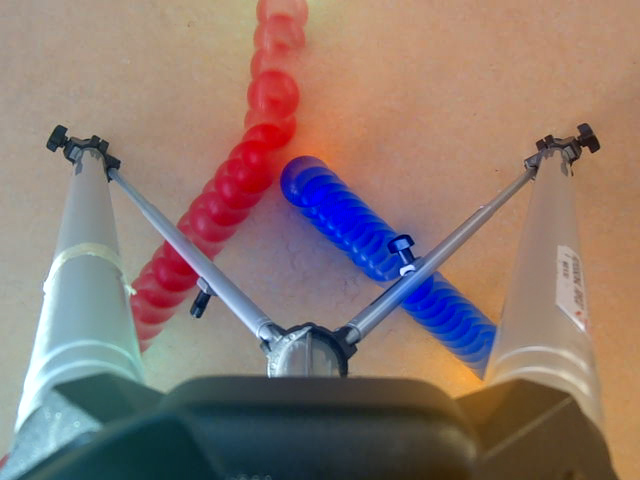
\includegraphics[width=0.45\textwidth]{Plaatjes/botsing3.jpg}}
		\,
		\subfloat[Simulatie met ons programma]{\label{botsing3-simulatie}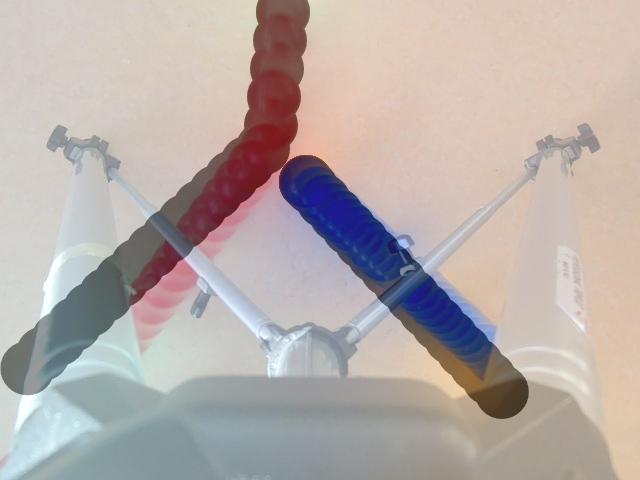
\includegraphics[width=0.45\textwidth]{Plaatjes/botsing3-simulatie.jpg}}
		\caption{Botsing tussen jeu de boules-ballen}
	\end{figure}

	Als we de resultaten met Coach uitlezen en in tabellen zetten, kunnen we er met Exel hieraan rekenen. Als we de positie uitzetten tegen de tijd krijgen we figuur \ref{00771} en \ref{00772}.
	
	\begin{figure}[H]
		\centering
		\subfloat[x-co\"{o}rdinaten]{\label{00771}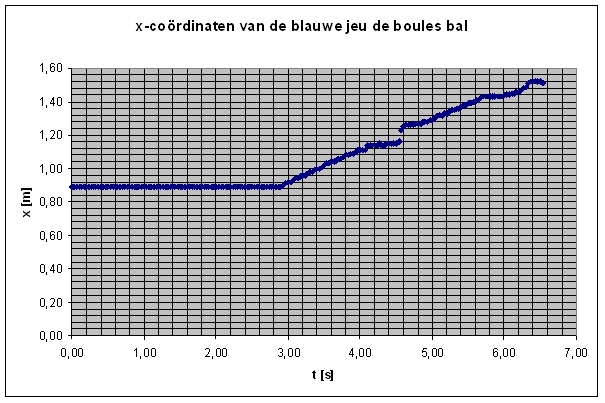
\includegraphics[width=0.45\textwidth]{Plaatjes/00771.png}}
		\,
		\subfloat[y-co\"{o}rdinaten]{\label{00772}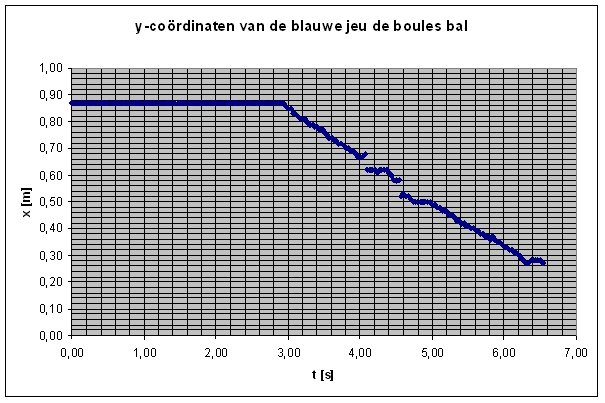
\includegraphics[width=0.45\textwidth]{Plaatjes/00772.png}}
		\caption{Co\"{o}rdinaten van de blauwe jeu de boules-bal}
	\end{figure}

	De blauwe bal licht in eerste instantie stil. Pas vanaf $t=2,94\ s$ begint de blauwe bal te rollen, nadat de rode bal er tegen aan is gebotst. Op ongeveer $t=4,30\ s$ tot $t=4,54\ s$ rolt de blauwe bal onder de paal door, hierdoor is het automatisch traceren op dit interval niet goed gelukt. Na $t=5,71\ s$ verdwijnt de bal uit het beeld, en is dus ook niet goed getraceerd. Als we dus alleen de goede meetresultaten mee rekenen krijgen we reeks \ref{00773} en \ref{00774}.
	
	\begin{figure}[H]
		\centering
		\subfloat[x-co\"{o}rdinaten (aangepast)]{\label{00773}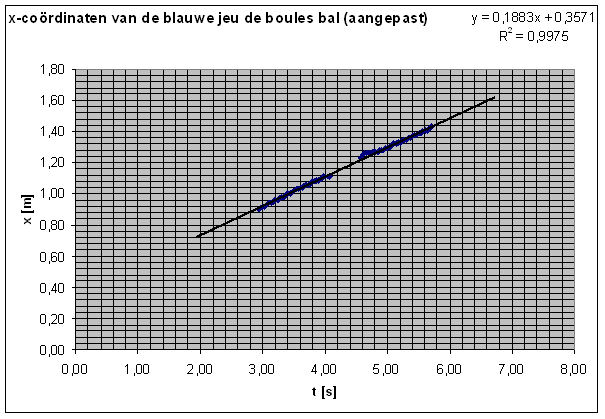
\includegraphics[width=0.45\textwidth]{Plaatjes/00773.png}}
		\,
		\subfloat[y-co\"{o}rdinaten (aangepast)]{\label{00774}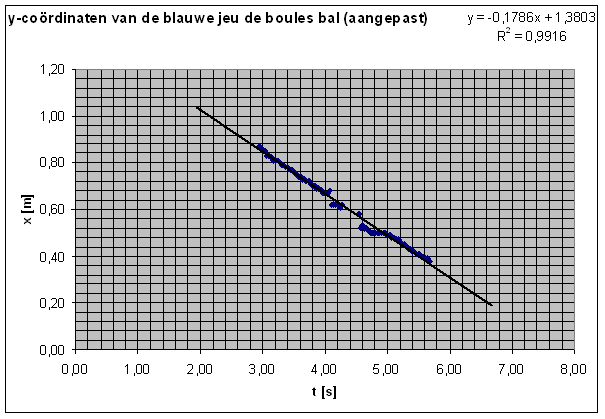
\includegraphics[width=0.45\textwidth]{Plaatjes/00774.png}}
		\caption{Co\"{o}rdinaten van de blauwe jeu de boules-bal}
	\end{figure}

	Nu hebben we de plaats in de $x$-richting en in de $y$-richting uitgezet tegen de tijd. Hieruit kunnen we de snelheid van de bal herleiden. Na $1,00\ s$ is de bal $0,1883\ m$ verplaatst in de $x$-richting en $0,1786\ m$ in de $y$-richting. De snelheid van de bal kun je dus berekenen met de $Stelling\ van\ Pythagoras$:

	\begin{equation}
		\label{snelheid}
		\begin{aligned}
			v&=\sqrt{{|rc_x|}^2+{|rc_y|}^2}\\
			v&=\sqrt{{rc_x}^2+{rc_y}^2}\\
		\end{aligned}
	\end{equation}

	De snelheid van de blauwe jeu de boules-bal na de botsing is dus: $v=\sqrt{{0,1883}^2+{0,1786}^2}=0,2595\ m/s$

	Nu hebben we de blauwe bal gehad, nu de rode bal. De rode bal heeft, in tegenstelling tot de blauwe, wel een begin snelheid. Omdat de rode bal heel weinig wordt afgebogen is het niet heel duidelijk te zien op werk tijdstip dit gebeurd. De bal wordt het meeste afgebogen in de $x$-richting, en als we in figuur \ref{00775} kijken kunnen we op $t=2,97\ s$ een verandering in de baan ontdekken.

	\begin{figure}[H]
		\centering
		\subfloat[x-co\"{o}rdinaten]{\label{00775}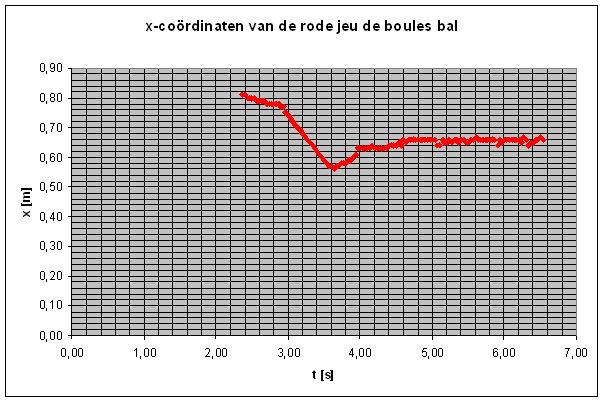
\includegraphics[width=0.45\textwidth]{Plaatjes/00775.png}}
		\,
		\subfloat[y-co\"{o}rdinaten]{\label{00776}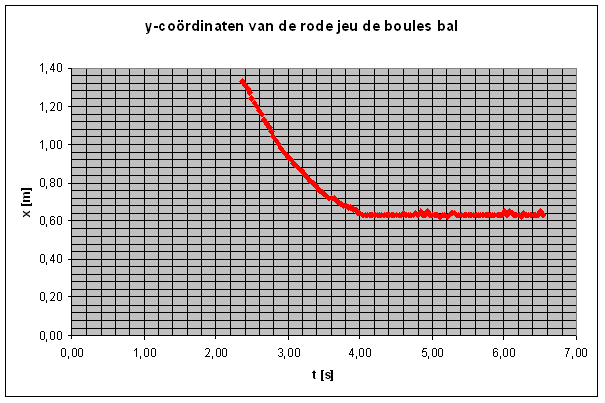
\includegraphics[width=0.45\textwidth]{Plaatjes/00776.png}}
		
		\caption{Co\"{o}rdinaten van de rode jeu de boules-bal}
	\end{figure}

	De punten van figuur \ref{00777} lijken een beetje vreemd, maar dat komt omdat we maar een klein aantal beeldjes hebben van de rode bal voor de botsing, de bal nauwelijk zich in de $x$-richting verplaatst en omdat het traceren niet nauwkeuriger gebeurt dan met twee decimalen.

	\begin{figure}[H]
		\centering
		\subfloat[x-co\"{o}rdinaten]{\label{00777}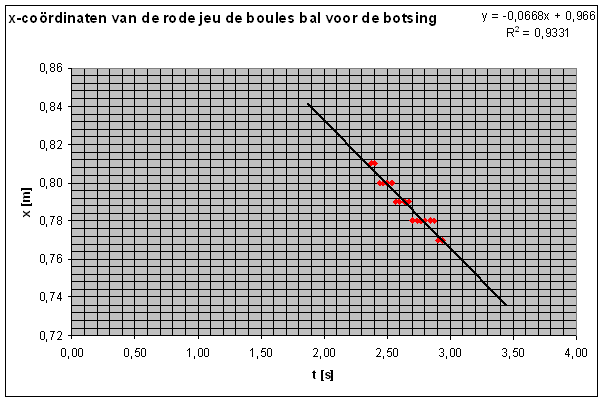
\includegraphics[width=0.45\textwidth]{Plaatjes/00777.png}}
		\,
		\subfloat[y-co\"{o}rdinaten]{\label{00778}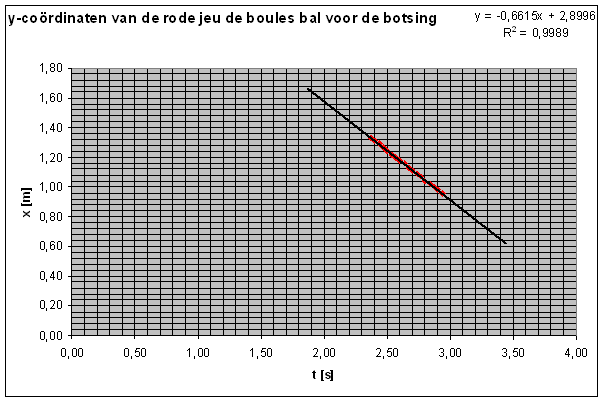
\includegraphics[width=0.45\textwidth]{Plaatjes/00778.png}}
		
		\caption{Co\"{o}rdinaten van de rode jeu de boules-bal voor de botsing}
	\end{figure}
	
	Hier doen we dus hetzelfde mee als met de blauwe jeu de boules-bal. De snelheid berekenen we dus met formule \eqref{snelheid}: $v=0,6649m/s$

	We hebben nu alleen nog maar de snelheid van de rode bal na de botsing nodig. Op figuur \ref{00775} is te zien dat de bal op $t=3,67\ s$ onder de paal door gaat en het traceren niet meer wil. Als we dus de meetresultaten van $t=2,79\ s$ tot $t=3,67\ s$ nemen krijgen we figuur \ref{00779} en \ref{007710}.

	We hebben nu alleen nog maar de snelheid van de rode bal na de botsing nodig. Op figuur \ref{00775} is te zien dat de bal op $t=3,67\ s$ onder de paal door gaat en het traceren niet meer wil. Als we dus de meetresultaten van $t=2,79\ s$ tot $t=3,67\ s$ nemen krijgen we figuur \ref{00779} en \ref{007710}.

	\begin{figure}[H]
		\centering
		\subfloat[x-co\"{o}rdinaten]{\label{00779}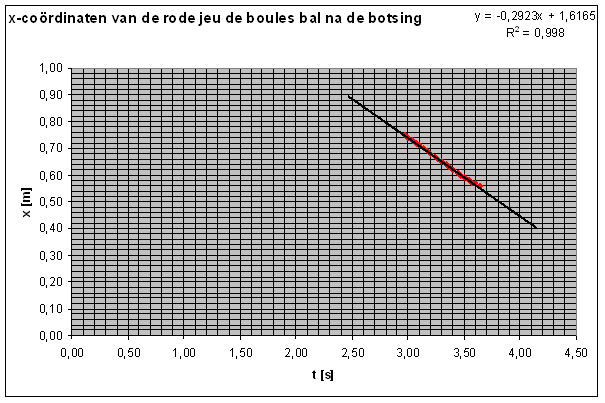
\includegraphics[width=0.45\textwidth]{Plaatjes/00779.png}}
		\,
		\subfloat[y-co\"{o}rdinaten]{\label{007710}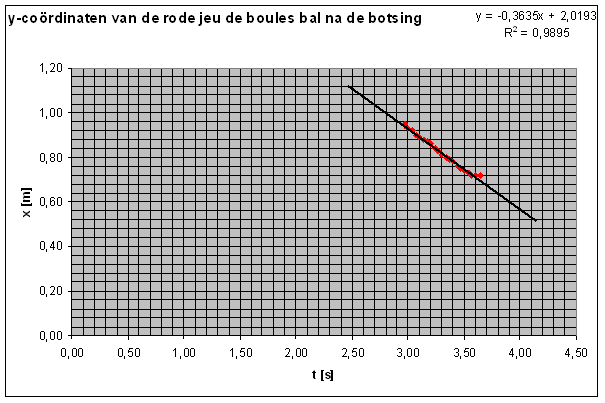
\includegraphics[width=0.45\textwidth]{Plaatjes/007710.png}}
		\caption{Co\"{o}rdinaten van de rode jeu de boules-bal na de botsing}
	\end{figure}
	
	De punten van figuur \eqref{00777} lijken een beetje vreemd, maar dat komt omdat we maar een klein aantal beeldjes hebben van de rode bal voor de botsing, de bal nauwelijk zich in de $x-richting$ verplaatst en omdat het traceren niet nauwkeuriger gebeurt dan met twee decimalen.

	Hier doen we dus hetzelfde mee als met de blauwe jeu de boules-bal. De snelheid berekenen we dus met formule \eqref{snelheid}: $v=0,6649m/s$

	We hebben nu alleen nog maar de snelheid van de rode bal na de botsing nodig. Op figuur \ref{00775} is te zien dat de bal op $t=3,67s$ onder de paal door gaat en het traceren niet meer wil. Als we dus de meetresultaten van $t=2,79s$ tot $t=3,67s$ nemen krijgen we figuur \ref{00779} en \ref{007710}.

	De snelheid hieruit berekenen geeft: $v=0,4664m/s$

	We stellen dat de blauwe bal, bal 1 is, en de rode bal, bal 2.
	Dan hadden we de volgende gegevens:

	\begin{tabular}{  l l }
		$m_1$= &0,22306 kg\\
		$m_2$= &0,22330 kg\\
		$o_1$= &0,0000 m/s\\
		$o_2$= &0,6649 m/s\\
	\end{tabular}

	Als het een centrale botsing zou zijn, dan zouden de snelheden na de botsing berekend kunnen worden met de formules van \eqref{uitwerking-energie-impuls}.
	$v_1$ zou in dat geval moeten zijn:

	\begin{equation}
		\begin{aligned}
			v_1&=\frac{\left(0,22306 \cdot 0,0000+0,22330 \cdot 0,6649\right)+0,22330 \cdot \left(0,6649-0,0000\right)}{\left(0,22306+0,22330\right)}=0,6653m/s\\
		\end{aligned}
	\end{equation}

	En $v_2$ zou moeten zijn:

	\begin{equation}
		\begin{aligned}
			v_2&=\frac{\left(0,22330 \cdot 0,6649+0,22306 \cdot 0,0000\right)+0,22306 \cdot \left(0,0000-0,6649\right)}{\left(0,22330+0,22306\right)}=0m/s
		\end{aligned}
	\end{equation}

	Maar in dit geval hebben we te maken met een niet-centrale botsing. Dus hebben we de posities nodig van de ballen op het moment van de botsing. De fotocamera maakte om de driehonderdste seconde een foto. Dit is niet genoeg om het exacte moment van de botsing te bepalen. Een kleine fout met Coach in het traceren kan grote afwijkingen hebben. De uitkomst zal waarschijnlijk ook niet helemaal overeenkomen met de werkelijkheid. In het programma zal dit beter lukken, omdat we daar met veel exactere waarden werken en er dus geen meetfouten, zoals met het traceren, kunnen ontstaan. En zoals blijkt uit figuur \ref{botsing3-simulatie}, klopt de simulatie met ons programma precies met de werkelijkheid, totdat de botsing plaatsvindt. De snelheden zijn ongeveer gelijk, maar de richting van de ballen is anders. Dit komt doordat ons programma werkt met compleet elastische botsingen, terwijl in realiteit dat soort botsingen amper bestaat.

	\newpage

	\section{Het eindproduct}
	Als eindproduct hebben we alle formules die we hebben opgesteld omgezet in een computerprogramma, waarmee we vrij nauwkeurige simulaties kunnen uitvoeren. We hebben gekozen voor een algemeen programma, waarmee mensen met kennis van programmeren zelf complexe simulaties kunnen maken en waarmee mensen zonder kennis van programmeren gemakkelijk simpele simulaties kunnen maken. Verder hebben we zelf een aantal voorbeelden gemaakt, om te laten zien wat de mogelijkheden zijn.
	
	Oftewel: de eindgebruiker maakt de simulatie, wij hebben de software gemaakt die de simulatie kan uitvoeren.
	
	\subsection{Wat er gesimuleerd kan worden}
	\begin{description}
  		\item[Voorwerpen] \hfill \\
  			Elk voorwerp heeft een positie. Verder zijn sommige voorwerpen statisch (onverplaatsbaar) en sommige dynamisch (verplaatsbaar).
			\begin{description}
				\item[Cirkel] \hfill \\
					De cirkel is een dynamisch voorwerp en heeft als extra eigenschappen een straal, een gewicht, een snelheidsvector en een lijst met krachten die erop werken.
				
				\item[Lijnstuk] \hfill \\
					Het lijnstuk is een statisch voorwerp en wordt voorgesteld als een vector.
			\end{description}
		\item[Krachten] \hfill \\
			Op elk dynamisch voorwerp kunnen oneindig veel krachten werken. Sommige krachten zijn constant, andere afhankelijk van de omstandigheden. Krachten worden weergegeven als vectoren.
			\begin{description}
				\item[Constante krachten] \hfill \\
					Constante krachten veranderen niet van grootte of richting, en blijven zoals ze in het begin van de simulatie zijn gedefinieerd. Een voorbeeld van een constante kracht is de zwaartekracht.
				\item[Afhankelijke krachten] \hfill \\
					Afhankelijke krachten kunnen veranderen van richting en grootte. Voorbeelden hiervan zijn spankracht en aantrekkingskracht tussen twee voorwerpen.
			\end{description}
		\item[Botsingen] \hfill \\
			Botsingen be\"{i}nvloeden de snelheidsvector van dynamische voorwerpen.
	\end{description}
	
	\subsection{Het programma}
	Voor het programma hebben we een aantal voorbeeldsimulaties gemaakt, die met de knoppen bovenaan te bekijken zijn.
	\begin{figure}[H]
		\centerline{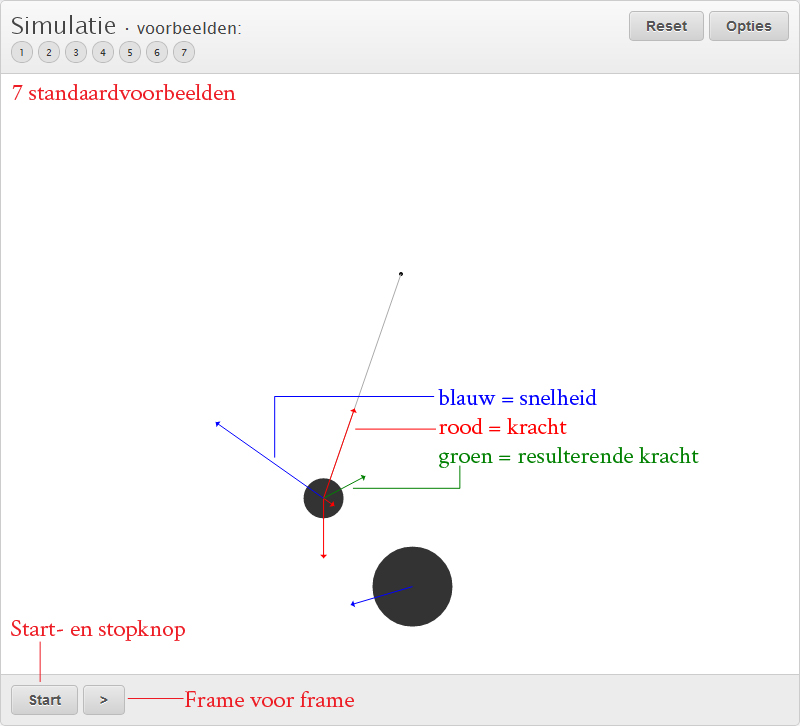
\includegraphics[width=\textwidth]{Plaatjes/programma-uitleg.jpg}}
		\caption{Een voorbeeld van een simulatie in het programma}
	\end{figure}
	Bij elke voorbeeldsimulatie zijn de basisgegevens te wijzigen, zoals positie, snelheid en massa.
	\begin{figure}[H]
		\centerline{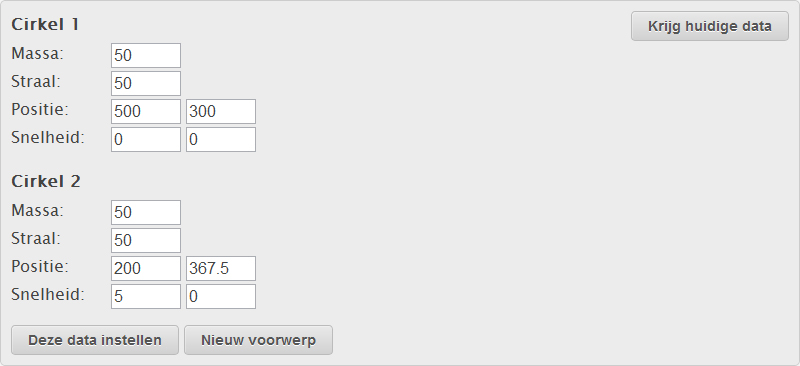
\includegraphics[width=\textwidth]{Plaatjes/programma-uitleg-instellen.jpg}}
		\caption{Instellingen veranderen en nieuwe voorwerpen toevoegen}
	\end{figure}
	
	\subsection{De werking van het programma}
	\label{werking-van-het-programma}
	Als een simulatie wordt uitgevoerd, leest ons programma eerst welke voorwerpen er zijn, welke eigenschappen die hebben en welke krachten er werken.
	
	Vervolgens voert de computer de volgende volgende stappen om de 30ms uit: 
	
	\begin{enumerate}
		\item Teken alle voorwerpen op het scherm;
		\item Bereken per voorwerp de resulterende kracht met behulp van $a = \tfrac{F_{res}}{m}$;
		\item Bereken per voorwerp de nieuwe snelheid;
		\item Kijk per voorwerp of het met een volgend voorwerp botst;
		\item Als er een botsing plaatsvindt:
			\begin{enumerate}
				\item Verplaats de twee voorwerpen naar botsingstand;
				\item Bereken de nieuwe snelheden;
				\item Onthoud hoeveel procent van de tijd tussen twee frames de botsende voorwerpen al hebben gebruikt
			\end{enumerate}
		\item Verplaats elk voorwerp met behulp van de snelheid
	\end{enumerate}
	
	We proberen de tijd tussen twee frames zo klein mogelijk te maken. Hoe kleiner de tijd tussen twee frames, des te betrouwbaarder de simulatie. Dit komt doordat we voor het berekenen van de snelheden en posities de definities voor versnelling en snelheid vrij letterlijk nemen:
	
	\begin{equation}
		\begin{aligned}
			\Delta \mathbf{v} = \Delta t \cdot \mathbf{a} \\
			\Delta \mathbf{x} = \Delta t \cdot \mathbf{v}
		\end{aligned}
	\end{equation}
	
	We stellen de tijd tussen twee frames als $\Delta t$, waardoor we voor het berekenen van de nieuwe snelheid domweg de versnelling kunnen optellen bij de snelheid, en op dezelfde manier de snelheid bij de positie kunnen optellen voor de nieuwe positie:
	
	\begin{equation}
		\begin{aligned}
			\mathbf{v} := \mathbf{v} + \mathbf{a} \\
			\mathbf{x} := \mathbf{x} + \mathbf{v}
		\end{aligned}
	\end{equation}
	
	\subsection{Voorbeeldcode voor complexe simulaties}
	Met ons programma kunnen andere mensen zonder verstand van botsingstheorie\"{e}n toch complexere simulaties uitvoeren door zelf te programmeren. Een voorbeeld daarvan is dit:
	
	\begin{lstlisting}[language=Javascript, caption={Vier cirkels, met een kracht op cirkel 1}]
// maak 2 cirkels

// Eerste cirkel: new Cirkel(straal, x, y)
var cirkel1 = new Cirkel(20, 20, 300);

// Beginsnelheid: 3px/frame naar rechts
cirkel1.snelheid = new Vector(3, 0);

// Constante kracht: 2px/frame naar rechts   
cirkel1.nieuweKracht( new Vector(2, 0) ); 
cirkel1.massa = 50;

// Tweede cirkel
var cirkel2 = new Cirkel(20, 100, 300);
cirkel2.massa = 50;

// Voeg ze toe aan de simulatie
wereld.nieuwVoorwerp(cirkel1);
wereld.nieuwVoorwerp(cirkel2);
	\end{lstlisting}

	\subsection{De grenzen van het programma}
	Natuurlijk verloopt een simulatie niet precies zoals het er in de werkelijkheid aan toe zou gaan. Er is nog een aantal natuurkundige zaken waar ons programma geen rekening mee houdt, en er is ook nog een technisch probleem. Bijvoorbeeld:
	\begin{description}
  		\item[Verlies van energie] \hfill \\
  			In ons programma zijn alle botsingen volkomen elastische botsingen, terwijl deze alleen theoretisch bestaan. Bij biljartballen is de hoeveelheid verloren energie aan wrijving verwaarloosbaar, maar er is toch zeker sprake van. Ons programma houdt dus geen rekening met het type stof, en gaat uit van onbuigbare volkomen harde stoffen.
		\item[Rotatie] \hfill \\
			Biljartballen die op elkaar botsen rollen, en hun botsing zal daarom een ander effect hebben dan dat van sjoelschijven of airhockeypucks. Ook treedt er rotatie op als een bal over een schuin lijnstuk rolt, wat niet verwerkt is in ons programma. Het gevolg in simulaties hiervan is, dat cirkels op een lijnstuk vast komen te zitten, in plaats van naar beneden te rollen.
		\item[E\'{e}n botsing per frame] \hfill \\
			Dit is misschien het meest vervelende probleem voor simulaties met veel snel bewegende voowerpen. Per frame kan hooguit het effect van \'{e}\'{e}n botsing worden berekend en gesimuleerd, waardoor er soms voorwerpen door elkaar heen vliegen.
	\end{description}
	
	\newpage

	\section{Conclusie}
	In dit profielwerkstuk zijn we erachter gekomen wat er bij botsingen gebeurt, hoe je dat in formules kunt uitdrukken en hoe je daar vervolgens simulaties van kan maken. Verder hebben we geleerd hoe je rekenwerk versimpelt, door gebruik te maken van vectoren.
	
	\subsection{Antwoorden op de deelvragen}
	Van tevoren hadden we ons een aantal vragen gesteld, die we nu kunnen beantwoorden.

	\subsubsection{Hoe werken botsingen bij poolballen?}
	Deze vraag hebben we algemener beantwoord; het antwoord is niet toegespitst op poolballen. Er is onderscheid tussen elastische en onelastische botsingen, en centrale en niet-centrale. Een botsing tussen een kogel en een zandzak is een voorbeeld van een onelastische botsing, en een poolbal met een andere poolbal is een voorbeeld van een bijna elastische botsing. Verder blijkt dat bij niet-centrale botsingen de snelheid in de richting van het botsingsvlak verandert, terwijl de snelheid evenwijdig aan het botsingsvlak gelijk blijft.

	\subsubsection{Met welke natuurkundige en wiskundige formules is de beweging te beschrijven?}
	Uiteindelijk bleken er vooral wiskundige formules gebruikt te worden voor het beschrijven van bewegingen. Dat komt vooral omdat natuurkundige formules moesten omschrijven, en we op zoek moesten naar tijdstippen van botsingen. Er zijn twee natuurkundige formules die we hebben samengevoegd om de snelheid na een botsing te bepalen, namelijk de formules over kinetische energie en impuls.

	\subsubsection{Hoe programmeer je deze formules?}
	Voor het programmeren heb je formules nodig met allerlei verschillende variabelen, die niet van tevoren ingevuld kunnen worden. Massa, positie, snelheid en krachten zijn per voorwerp anders, en dus hadden we algemene formules nodig. Als je die formules eenmaal hebt, is er geen kunst aan om ze te programmeren, omdat je de eigenschappen per voorwerp in \'{e}\'{e}n object kunt verwerken, en de formules bijna letterlijk kunt overtypen. We moesten wel van tevoren alle basisbewerkingen van vectoren programmeren, maar dat was ook niet al te lastig.

	\subsubsection{Hoe optimaliseer je de snelheid van het programma?}
	Met gebruik van vectoren hebben we alle formules korter kunnen schrijven, zodat de hoeveelheid code klein blijft. Daarmee kun je sneller programmeren, maar dat zegt niets over de snelheid van het programma. Een bijkomstigheid van het werken met vectoren was, dat we door de eigenschappen van het inproduct \eqref{inproduct-cosinus} op geen enkele plek een sinus, cosinus of tangens hebben gebruikt. Zoals gezegd zijn die functies relatief tijdrovend voor de computer. Nog een voorbeeld van kleine snelheidsoptimalisatie is de aangepaste ABC-formule \eqref{a2bc}, voor vergelijkingen met de vorm $ax^2+2bx+c=0$.
	
	Al met al schokt het programma niet, zelfs niet als je meer dan tien voorwerpen simuleert.
	
	\newpage
	
	\section{Nawoord}
	Tijdens het maken van het profielwerkstuk hebben we opvallend veel nieuwe zaken geleerd, zowel in de natuurkunde als in de wiskunde. Dit profielwerkstuk was duidelijk een verbreding, waarin we een duik namen in de botsingstheori\"{e} en het nodige leerden over werken met vectoren.
	
	Daarnaast hebben we ook opvallend veel technische zaken geleerd, zoals het werken met \LaTeX. Ons hele verslag is hierin geschreven, zodat we makkelijker de opmaak van formules konden instellen. Voor de plaatjes leerden we gebruikmaken van GeoGebra, wat toch wel mooie resultaten opleverde. Om het simulatieprogramma te schrijven hebben we gebruikgemaakt van een zeer nieuwe techniek, namelijk een combinatie van HTML5 en Javascript. Alle simulaties zouden daarom zo op internet kunnen komen te staan, maar het is nog wachten op de volledige implementatie van deze techniek in de huidige webbrowsers. Het meest ingewikkelde was toch wel het werken met Git. Met Git kun je met meerdere personen werken aan \'{e}\'{e}n tekstbestand, waarbij alle veranderingen terug te draaien zijn, zonder dat er ook maar iets van wat geschreven is verloren kan gaan.
	
	Kortom, we hebben ontzettend veel geleerd, de samenwerking ging redelijk goed, en we hebben al met al een aardig mooi eindproduct gemaakt.

\end{document}